\chapter{Building a Linux Filesystem}\label{disk-fs}

\textbf{XXX---add proc\_create\_single() call and display files accessed by walking through the inode list}

There are two ways to understand filesystems. Either you can study one of more of the 80+ existing filesystems or you can develop one. The issue with studying existing filesystems is that they all have their peculiarities which 
make analyzing the source code more complicated. For example, I’ve looked at BFS which is a simple filesystem developed for UNIX SVR4 (System V Release 4) for the \cf{/stand} filesystem. It’s a filesystem I worked with many years ago. It only has 1200 lines of kernel source code but still has a few twists. It’s background:

It was designed to hold all binaries needed during the boot phase. It’s simple disk layout helped with simplifying the boot loader which didn’t need to know about the structure of more complex filesystems such as UFS and VxFS which were commonplace on SVR4 at the time. As such it was not designed for general purpose usage.

\begin{itemize}
	\item It’s a flat filesystem (only files within a single root directory). 
	\item Only regular files can be created. You can't create symbolic links.
	\item Files are allocated contiguously, again to simplify boot. This makes writing files more complex 
		since blocks need to be moved to retain this requirement.
	\item XXX - anything else?
\end{itemize}

\noindent
It would be better to have a simple filesystem without these limitations but with a goal of keeping it about the same size in terms of lines of code. I developed such a filesystem for my first book (UNIX Filesystems - Design and 
Implementation) in 2003 for the Linux 2.4 kernel. I’ve used that as a base (things have changed quite a bit since) but hopefully made it easier to understand by adding more tracing and fixing some bugs that slipped under the 
rug. This new filesystem is called SPFS (no prizes for guessing the name).

Here are the main characteristics of SPFS:

\begin{itemize}
	\item Multi-level directories (directories within directories)
	\item Fixed block size (2048 bytes).
	\item A filename length up to 28 characters.
	\item 760 blocks within the whole filesystem.
	\item A maximum file size of approximately 505 KB.
	\item File undelete using the SPFS \cf{fsdb} command.
	\item File creation, deletion, rename, ... \cf{XXX}
\end{itemize}

\noindent
Most of these limitations are in place to keep the on-disk structures very simple which result in the code to access them being much easier to understand. The goal here is for teaching.

\section{The SPFS on-disk Format}

As discussed earlier, simplicity is key. We are not trying to design a high-performing, crash-resistant filesystem but one with the simplest structure and the least amount of code (around 2,000 lines including \cf{mkfs}, \cf{fsdb} and lots of debug messages and debug ioctls.

The filesystem block size for SPFS is 2-38 bytes. If we have a regular file with size of 0, it will have no allocated blocks. If the size of the file is <= 2048 bytes it will have 1 block. If the size of the file is 2049 bytes it will have 2 blocks allocated and so on. The same is true for directories. There is never an empty directory because a newly allocated directory will always have entries for "." and "..". Directory entries are 32 bytes so a new directory will have one allocated 2048 byte block and a size of 64 bytes.

The superblock is limited to one block due to the way superblocks are accessed as part of mount processing. Since this structure maintains a list of used/unused inodes and blocks in the filesystem, this is where our limitation of the filesystem size and number of files comes from. To increase the size of the superblock beyond 1024 bytes would add additional complexity which we are trying to avoid.

There are three components to the disk layout as shown in figure \ref{fig:fslayout}.

\begin{figure}
	\centering
	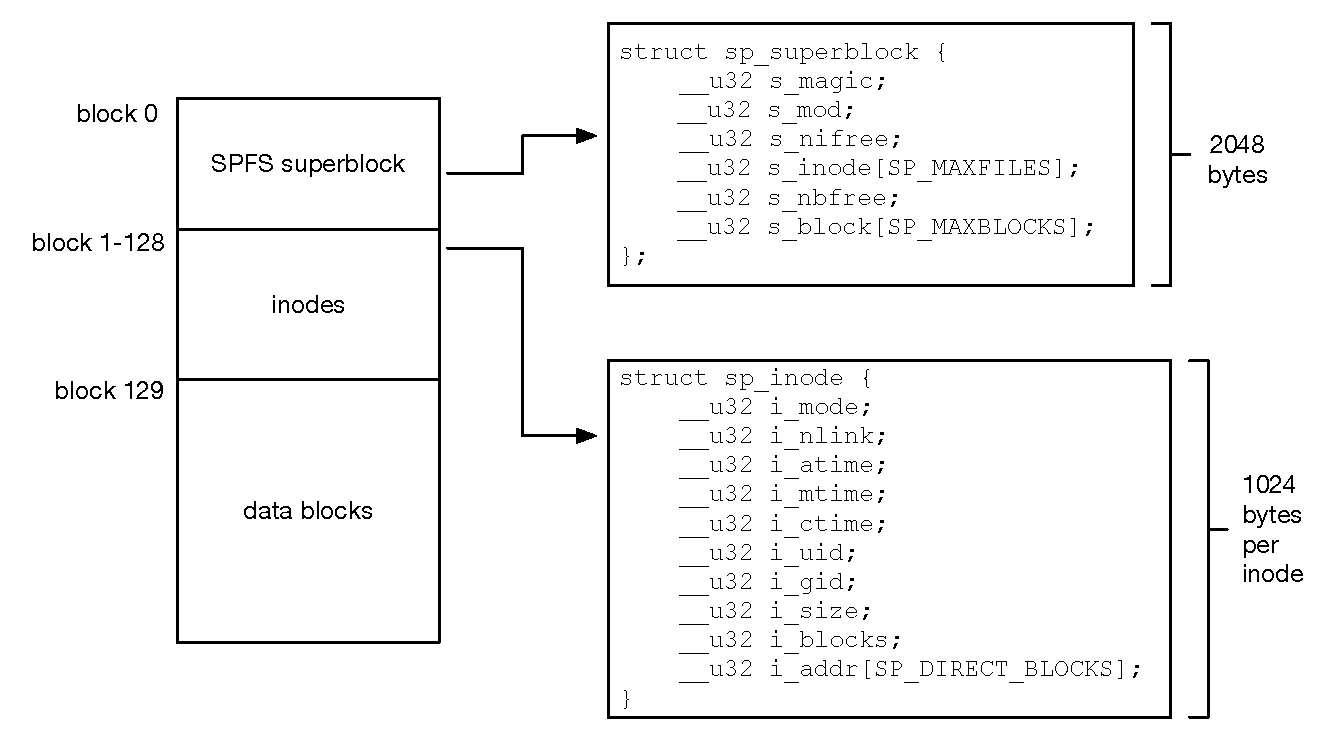
\includegraphics[scale=0.56]{figures/fslayout.pdf}
	\caption{Filesystem layout on disk}
	\label{fig:fslayout}
\end{figure}

\begin{enumerate}
	\item \textbf{Superblock} --- this is stored in block 0.
	\item \textbf{Inodes} --- stored in blocks 1-128. There is one inode per block. This is very inefficient in terms of 
		space but as we shall see later, locating the block where the inode is stored is very simple. It’s just 
		block 1 + inode number. For example, the root inode is stored at block 3. There can only be 128 files in 
		the filesystem and since inodes 0, 1 aren't used and inode 2 is for the root directory, a maximum of
		124 new files that can be created.
	\item \textbf{Data blocks} --- stored from block 129 onwards. Data blocks are used for regular file data as well 
		and directory entries for directories and symbolic links. 
\end{enumerate}

%%%%%%%%%%%%%%%%%%%%%%%%%%%%%%%%%%%%%%%%%%%%%%%%%%%%%%%%%%%%%%

\section{A Note About Printing Pointers}

There are several places in the code where I print out pointers. This helps with debugging. If structures are still valid, I can drop into \cf{gdb} and display them easily. If you make a call such as:

\begin{lstlisting}
printk("*** set i_private to \%p\n", spi);
\end{lstlisting}

\noindent
you will a message something along the lines of:

\begin{lstlisting}
*** set i_private to 00000000aa1e52ff
\end{lstlisting}

\noindent
which is not a valid address. You should be seeing an address more along the lines of:

\begin{lstlisting}
*** set i_private to ffff0000c98dd470
\end{lstlisting}

\noindent
This is because an address printed with \cf{\%p} will first be hashed to prevent the real address from being exposed. On 64-bit machines, the first 32 bits are zeroed before printing as seen above.

To see the real address, use \cf{\%px} in place of \cf{\%p}. For development purposes this is fine but for production code, be well aware of what you're printing in case there are potential security issues with exposing kernel addresses.

%%%%%%%%%%%%%%%%%%%%%%%%%%%%%%%%%%%%%%%%%%%%%%%%%%%%%%%%%%%%%%

\section{From Module Load to Mounting a Filesystem}

In \ref{fig:module-load} we show which functions are called as part of loading the module (and unloading) and how the filesystem’s mount function is identified to the kernel and called.

\begin{figure}
	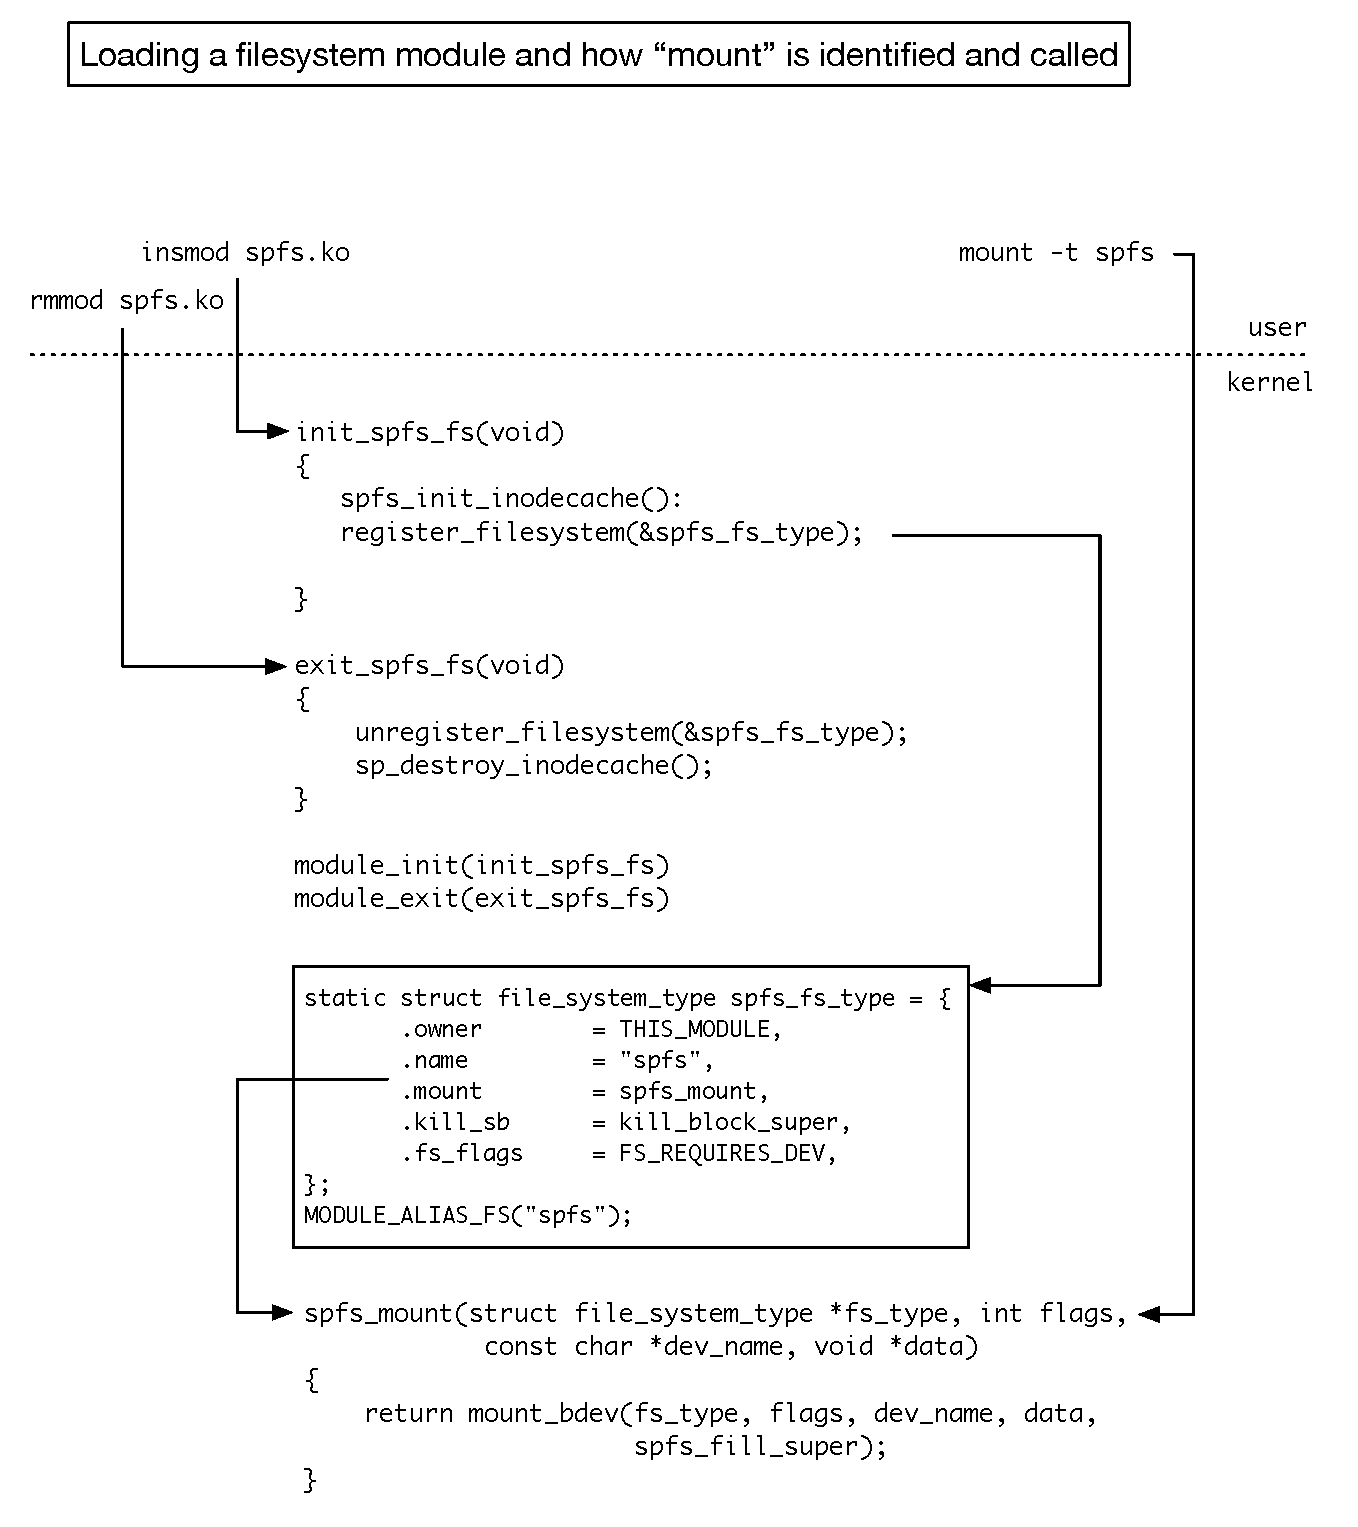
\includegraphics[scale=0.45]{figures/module-load.pdf}
	\centering
	\caption{Module Initialization}
	\label{fig:module-load}
\end{figure}

First of all we declare our filesystem module through the \cf{file\_system\_type} structure (shown in gray). Here we have:

\begin{itemize}
	\item The name of the filesystem.
	\item The filesystem’s \cf{mount} function that should be called when a filesystem of type \cf{spfs} 
	         is mounted (\cf{mount -t spfs}).
	\item The function that should be called during \cf{umount } processing to clean up everything. 
		XXX - need to figure out if anything is left other than setting the SB to CLEAN and flushing it.
\end{itemize}

\noindent
There are two functions declared:

\begin{itemize}
	\item \cf{init\_spfs\_fs()} - this will be called when the module is loaded (either 
		\cf{insmod} or \cf{mount -t spfs} - XXX need to figure out the MODULE\_ALIAS\_FS(“spfs") stuff
	\item \cf{exit\_spfs\_fs()} - this is called when the module is unloaded (\cf{rmmod}).
\end{itemize}

\noindent
When the module is loaded, the first thing that \cf{init\_spfs\_fs()} performs is to register the file system by calling \cf{register\_filesystem()}. The main goal of this function is to check that the filesystem has not already been registered. If not, it is added to the list of available filesystems as shown in figure \ref{fig:filesystems-available} . XXX - need to check this with a debugger to show how many filesystems and make sure spfs is last on the list.

\begin{figure}[h]
	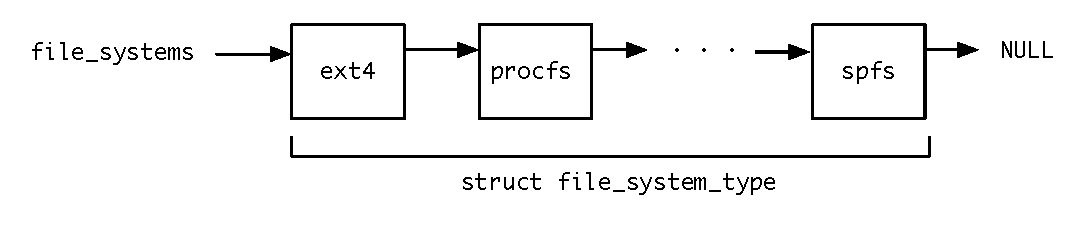
\includegraphics[scale=0.6]{figures/filesystems-available.pdf}
	\centering
	\caption{The list of available Linux filesystems that can be mounted}
	\label{fig:filesystems-available}
\end{figure}

The \cf{file\_systems} variable can be found in the file \cf{fs/filesystems.c} next to \cf{register\_filesystem()} and associated functions.

When issuing a \cf{mount -t spfs} call, the kernel can walk through this list checking the \cf{spfs} argument against the name field of each \cf{file\_system\_type} structure in the list. If there is a match, the kernel can locate the filesystem-specific mount function and call it.

%%%%%%%%%%%%%%%%%%%%%%%%%%%%%%%%%%%%%%%%%%%%%%%%%%%%%%%%%%%%%%

\section{Initializing the per-filesystem Inode Cache}

Every filesystem has its own \cf{init\_inodecache()} function for maintaining a list of per-filesystem inodes (all mounts?). When allocating a Linux inode, a call is made to \cf{alloc\_inode\_sb()} (linux/fs.h) where they say:

\begin{quote}
\it This must be used for allocating filesystems specific inodes to set up the inode reclaim context correctly.
\end{quote}

\noindent
When creating or opening a file, a Linux inode is created. There is one inode regardless of the number of open file descriptors. To populate many of the fields of the inode, the kernel requests the filesystem to allocate the inode. For existing files, this involves reading the corresponding SPFS inode from disk. Much of the information about the file is used to populate the Linux inode but there is some information that SPFS must also keep in-core. This information relates to where the data blocks for the file are stored on disk (all file types---regular, directories and symlinks) and how many blocks have been allocated so far.

Here is both the SPFS in-core inode and the SPFS disk inode. The Linux inode is embedded within the SPFS in-core inode. All inodes for this mounted filesystem are referenced from the \cf{super\_block} structures as shown in figure \ref{fig:inode-lru-list}. When a \cf{sp\_inode\_info} structure is allocated, we store "SPFS" in the \cf{i\_fs} field. This is just for debugging purposes to show the structure type. It will be shown in different KGDB demonstration sessions throughout the book.

\begin{lstlisting}
struct sp_inode_info {
    char            i_fs[4];
    int             i_blocks;
    int             i_addr[SP_DIRECT_BLOCKS];
    char            i_symlink[SP_NAMELEN];
    struct inode    vfs_inode;  
};
\end{lstlisting}

\noindent
The disk-based inode contains more fields. All but the last two fields are copied to the Linux inode so there is no point replicating them in the in-core SPFS inode.

\begin{lstlisting}
struct sp_inode {
	__u32	i_mode;
	__u32	i_nlink;
	__u32	i_atime;
	__u32	i_mtime;
	__u32	i_ctime;
	__u32	i_uid;
	__u32	i_gid;
	__u32	i_size;
	__u32	i_blocks;
	__u32	i_addr[SP_DIRECT_BLOCKS];
};

#define ITOSPI(inode) (struct sp_inode_info *)&inode->i_private
\end{lstlisting}

\begin{figure}
	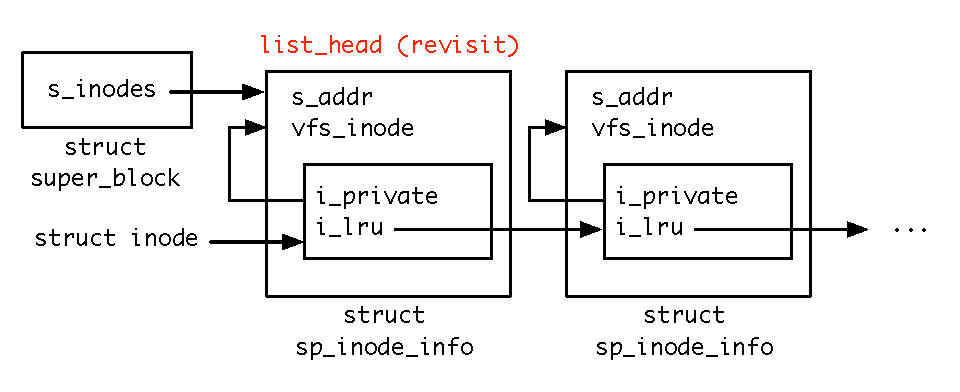
\includegraphics[scale=0.6]{figures/inode-lru-list.pdf}
	\centering
	\caption{Inode LRU List referenced from the \cf{super\_block} structure}
	\label{fig:inode-lru-list}
\end{figure}

\noindent
Many calls into SPFS pass the Linux inode. We often need to access the SPFS in-core inode which we can do through use of the \cf{ITOSPI()} macro. We'll discuss how this LRU list is used later on in the book XXX.

%------------------------------------------------------------------------------------------------------------------------------------------------------------------------

\subsection{KGDB - Analyzing Inode Lists for a Specific Mountpoint}\label{kdgb-inodelist}

Section \ref{container-of} describes how the \cf{container\_of()} inline function is used to located a structure given an element within the containing structure The previous section described how this is used for Linux VFS inodes and SPFS inode information. In this section we'll describe how to analyze inode lists associated with a specific mount point.

First, we'll show how to walk the list by hand in \cf{gdb} which is quite painful, especially if there are a lot of elements in the list. We'll then combine this approach with \cf{crash} which makes walking linked lists much easier. \textbf{XXX---can we do this for for\_each() or something like that??? - or write some gdb scripts at some point.}

The goal is to walk the inode list and located an inode that matches a specific file. Here are the files in the filesystem being used. We'll located \cf{file-3} which has an inode number of \cf{6}.

\begin{lstlisting}
$ [*\bfseries ls -li /mnt*]
total 1
4 -rw-r--r-- 1 root root  0 Feb  7 17:26 file-1
5 -rw-r--r-- 1 root root  0 Feb  7 17:26 file-2
6 -rw-r--r-- 1 root root  0 Feb  7 17:26 file-3
3 drwxr-xr-x 2 root root 64 Feb  7 17:26 lost+found/
\end{lstlisting}

\noindent
All mounted filesystems are on a doubly linked list headed by the \cf{super\_blocks} global variable:

\begin{lstlisting}
(gdb) [*\bfseries p super\_blocks*]
$1 = {next = 0xffff0000c0020800, prev = 0xffff0000cdc18000}
\end{lstlisting}

\noindent
Looking at the top of the \cf{super\_block} structure (one per mounted filesystem) we can see that the \cf{s\_list} field keeps all such structures in a linked list:

\begin{lstlisting}
struct super_block {
    struct list_head    s_list;     /* Keep this first */
    ...
}
\end{lstlisting}

\noindent
Thus the two addresses shown above are the addresses of the first \cf{super\_block} in the list and also the last one.

Inodes are different in that the list is embedded part way down the inode structure so we will need to use \cf{container\_of()} to get to the actual inode whereas we can use the addresses above directly to reference the \cf{super\_block} structure.

\begin{lstlisting}
struct inode {
    ...
    struct list_head    i_sb_list;
    ...
}
\end{lstlisting}

\noindent
We're going to look at the last filesystem mounted so we can look at the \cf{super\_block} structure shown by \cf{prev} and get the inode list which is stored in the \cf{s\_inodes} field. Take note of the first address in bold (\cf{0xffff000004418518}) which is the first inode in the list and when it is shown later when printing out \cf{\$14}. In the second case it's the \cf{next} element in the double linked list shown that we've walked through the whole list.

\begin{lstlisting}
(gdb) [*\bfseries p ((struct super\_block *)0xffff0000cdc18000)->s\_inodes*]
$5 = {
  next = [*\bfseries 0xffff000004418518,*]
  prev = 0xffff0000044f3f98
}
\end{lstlisting}

\noindent
Now the fun begins! We walk this list by hand from the head of the list to the tail. Luckily it's actually a very short list.

\begin{lstlisting}
(gdb) [*\bfseries p ((struct list\_head *)0xffff000004418518)->next*]
$6 = (struct list_head *) 0xffff0000b38e1f18
(gdb) [*\bfseries p *\$6*]
$9 = {
  next = 0xffff0000b38e3918,
  prev = 0xffff000004418518
}
(gdb) [*\bfseries p ((struct list\_head *)0xffff0000b38e3918)->next*]
$12 = (struct list_head *) 0xffff0000b38e2598
(gdb) [*\bfseries p *\$12*]
$13 = {
  next = 0xffff0000044f3f98,
  prev = 0xffff0000b38e3918
}
(gdb) [*\bfseries p ((struct list\_head *)0xffff0000044f3f98)->next*]
$14 = (struct list_head *) 0xffff0000cdc18588
(gdb) [*\bfseries p *\$14*]
$15 = {
  next = [*\bfseries 0xffff000004418518*],
  prev = 0xffff0000044f3f98
}
\end{lstlisting}

\noindent
Let's pick one of these addresses, say \cf{0xffff000004418518} which is highlighted. We can use \cf{container\_of()} go go from this address to the address of the inode in question. Here is the call. This particular inode list is referenced from the \cf{i\_sb\_list} field of the inode structure so we pass this address, the structure type and the structure element name for which the address applies:

\begin{lstlisting}
(gdb) [*\bfseries set \$inode = *\$container\_of(0xffff000004418518,*] \
[*\bfseries "struct inode", "i\_sb\_list")*]
\end{lstlisting}

\noindent
Now we have the inode, we can print out the inode number which matches the inode number displayed when running \cf{ls} earlier.

\begin{lstlisting}
(gdb) [*\bfseries p \$inode.i\_ino*]
$19 = 6
\end{lstlisting}

\noindent
Getting to a \cf{dentry} structure to find the filename requires another call to \cf{container\_of()} since there could be a list of dentries (if there were hard links to the same file and more than one was accessed). First thing is to located the list inside the inode:

\begin{lstlisting}
(gdb) [*\bfseries p \$inode.i\_dentry.first*]
$23 = (struct hlist_node *) 0xffff0000b3b409b0
\end{lstlisting}

\noindent
and then call \cf{container\_of()} again to get the first dentry:

\begin{lstlisting}
(gdb) [*\bfseries set \$dentry = *\$container\_of(0xffff0000b3b409b0, *] \
[*\bfseries "struct dentry", "d\_u")*]
\end{lstlisting}

\noindent
The \cf{dentry} structures are also linked as follows which is why we use the \cf{d\_u} field.

\begin{lstlisting}
struct dentry {
    ...
    union {
        struct hlist_node d_alias;  
        struct hlist_bl_node d_in_lookup_hash;  
        struct rcu_head d_rcu;
    } d_u;
} __randomize_layout;
\end{lstlisting}

\noindent
Now we have our dentry, we can display the file name:

\begin{lstlisting}
(gdb) [*\bfseries pipe p \$dentry | grep 'name = "'*]
  d_iname = "file-3", '\000' <repeats 25 times>,
\end{lstlisting}

\noindent
A bettter alternative to walking Linux kernel linked lists by hand is to define a \cf{gdb} function to do the work for us.

\begin{lstlisting}
define plist
  set var $n = $arg0->head
  while $n
    printf "%d ", $n->data
    set var $n = $n->next
  end
end
\end{lstlisting}

\noindent
\textbf{XXX---this does not work! At least I've tried it and it doesn't work. Python may be a better choice}

% https://kernel.googlesource.com/pub/scm/linux/kernel/git/mchehab/linux-media/+/media/v4.7-2/scripts/gdb/linux/lists.py - a list of useful scripts

The \cf{crash(1)} command has a nice command to walk through lists so rather than the previous example in \cf{gdb} where we walked through by hand, one command does it in \cf{crash}. First of all, we follow the same path as the earlier example of finding the last mounted filesystem to get its \cf{super\_block} structure and from there, find the list of inodes. In this example, we have a different filesysytem. Here are the files in the \cf{/mnt} directory:

\begin{lstlisting}
$ [*\bfseries ls -li /mnt*]
total 28
15 -rw-r--r-- 1 root root     6 Feb  8 19:03 file-1
14 -rw-r--r-- 1 root root     6 Feb  8 19:04 file-2
16 -rw-r--r-- 1 root root     6 Feb  8 19:03 file-3
11 drwx------ 2 root root 16384 Feb  3 15:51 lost+found/
\end{lstlisting}

\noindent
The first step is to find the list of \cf{super\_block} structures and, knowing that this was the last filesystem mounted, use the \cf{prev} field, display the \cf{super\_block} structure for this filesystem and get the list of associated inodes:

\begin{lstlisting}
crash> [*\bfseries super\_blocks*]
super_blocks = $2 = {
  next = 0xffff5a09c0026000,
  prev = 0xffff5a09d2fcb000
}
crash> [*\bfseries super\_block 0xffff5a09d2fcb000*]
  ...
  s_inodes = {
    next = [*\bfseries 0xffff5a09d3ffb950*],
    prev = 0xffff5a09d3ff86c8
  },
  ...
\end{lstlisting}

\noindent
Using the head of the list (shown in bold), the \cf{list} command is called to display all entries. Magical!

\begin{lstlisting}
crash> [*\bfseries list 0xffff5a09c1f27318*]
ffff5a09d3ffb950
[*\bfseries ffff5a09c0ef8ff8 *]
ffff5a09c0eff070 
ffff5a09197f79a0 
ffff5a09d3ffa6f0
ffff5a09d3ff9dc0
ffff5a09d3ff86c8
ffff5a09d2fcb548
\end{lstlisting}

\noindent
I've already looked at some of the inodes to find out which ones correspond to our files so picking the address highlighted, here is teh equivalent of calling \cf{container\_of()} in \cf{gdb}. The \cf{-l} option tells \cf{crash} to display the containing inode structure using the structure element \cf{i\_sb\_list} as a field within this structure.

\begin{lstlisting}
crash> [*\bfseries inode -l inode.i\_sb\_list ffff5a09c0ef8ff8*]
...
  i_ino = 14,
  {
    i_nlink = 1,
    __i_nlink = 1
  },
  i_rdev = 0,
  i_size = 6,
      ...
    i_dentry = {
      first = 0xffff5a0900dc10b0
    },
...
\end{lstlisting}

\noindent
You can now see the inode number and file size which matches \cf{file-2} displayed by \cf{ls} above. To confirm the file name, we need to use the same technique to find the \cf{dentry} structure:

\begin{lstlisting}
crash> [*\bfseries dentry -l dentry.d\_u 0xffff5a0900dc10b0*]
  d_name = {
    {
      {
        hash = 2573278399,
        len = 6
      },
      hash_len = 28343082175
    },
    name = 0xffff5a0900dc1038 "file-2"
  },
  d_inode = 0xffff5a09c0ef8ee0,
  d_iname = "file-2\000\0 ... 000\000",
\end{lstlisting}

\noindent
This is quite a bit simpler than walking the linked list by hand with \cf{gdb} but is otherwise very similar.

%%%%%%%%%%%%%%%%%%%%%%%%%%%%%%%%%%%%%%%%%%%%%%%%%%%%%%%%%%%%%%%%

\section{Mounting a Filesystem}

When a filesystem is mounted, the filesystem type is passed as an argument, for example:

\begin{lstlisting}
# [*\bfseries mount -t spfs /dev/sdb1 /mnt*]
\end{lstlisting}

\noindent
The kernel uses this argument to find the correct \cf{file\_system\_type} structure (see figure \ref{fig:filesystems-available}) and call the filesystem’s mount function. Recall that this is one of the fields in struct \cf{file\_system\_type} and was passed to the kernel during module load by calling \cf{register\_filesystem()}.

Here are the set of calls (viewable using \cf{dmesg}) made from the kernel into SPFS to complete the mount call. The root inode of the filesystem is inode 2.

\small
\bigskip
\cf{spfs\_mount()} $\rightarrow$ \cf{spfs\_fill\_super()}  $\rightarrow$ \cf{sp\_read\_inode()}
%\\~\\

\bigskip
\normalsize
\noindent
Following a call to mount, any operation on this filesystem must start with the root directory and thus, the kernel will call the \cf{read\_inode()} function in the \cf{super\_operations} structure to read the root inode in from disk.

Xxx - Need a figure of kernel structures for this

%------------------------------------------------------------------------------------------------------------------------------------------------------------------------

\subsection{Inside \cf{sp\_mount} and \cf{sp\_fill\_super}}

The code for \cf{spfs\_mount()} is very simple, relying solely on a call to \cf{mount\_bdev()}. It passes \cf{spfs\_fill\_super()} as as argument.

\begin{lstlisting}
static struct dentry *
[*\bfseries spfs\_mount*](struct file_system_type *fs_type, int flags, 
			   const char *dev_name, void *data)
{
    return [*\bfseries mount\_bdev*](fs_type, flags, dev_name, data, 
                      [*\bfseries spfs\_fill\_super*]);
}
\end{lstlisting}

\noindent
After calling \cf{spfs\_fill\_super()},  figure \ref{fig:per-mount-structures} shows how the structures are linked together.

\begin{figure}
	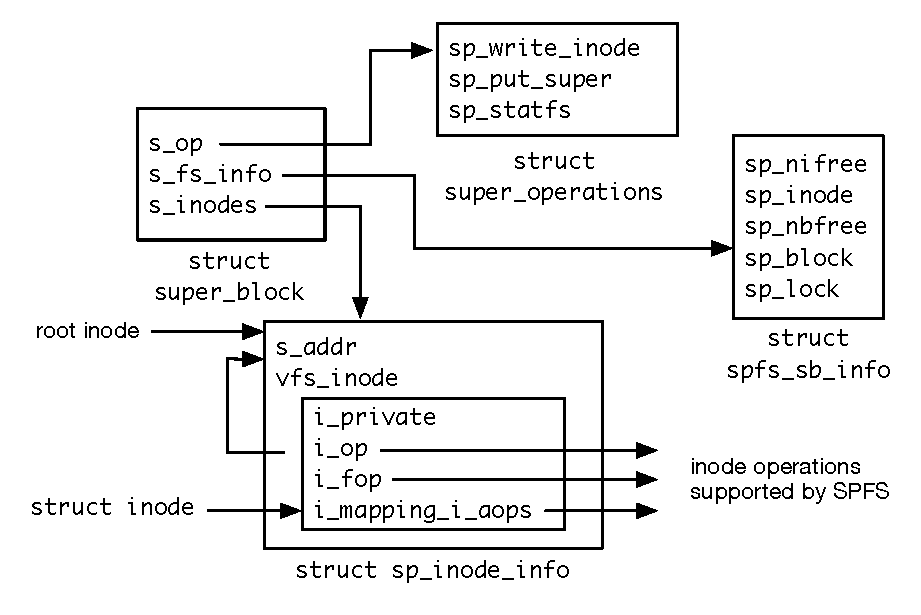
\includegraphics[scale=0.6]{figures/sp_fill_super.pdf}
	\centering
	\caption{Per-mount structures following a call to \cf{sp\_fill\_super()}}
	\label{fig:per-mount-structures}
\end{figure}

At this point we have enough structure in place to allow us to do the following type of operations:\textbf{XXX---we can do more than this so elaborate}

\begin{itemize}
	\item Get filesystem information (think about calling the \cf{df(1)} command) through use of 
		 the \cf{sp\_statfs()} function.
	\item List the contents of the root directory.
	\item Lookup files in a specified directory.
\end{itemize}

\noindent
As we progress through the filesystem, more inodes will be read into memory and from there we can perform all the basic filesystem operations. XXX - we’ll expand …

For the moment, let’s look more at \cf{sp\_fill\_super()} ...

%%%%%%%%%%%%%%%%%%%%%%%%%%%%%%%%%%%%%%%%%%%%%%%%%%%%%%%%%%%%%%%

\section{SPFS super\_operations}

So we have a separation from mount and unmount (see module loading section below)

\begin{lstlisting}
static const struct super_operations spfs_sops = {
	.alloc_inode. = sfs_alloc_inode,
	.free_inode.  = sfs_free_inode,
	.write_inode  = sfs_write_inode,
	.evict_inode  = sfs_evict_inode,
	.put_super    = sfs_put_super,
	.statfs       = sfs_statfs,
};
\end{lstlisting}

\noindent
Any of the operations that your filesystem provides are called by the kernel once the filesystem is mounted.

bfs\_put\_super() doesn’t do much other than free the structure. I guess because this is a read-only FS? It was similar for uxfs which is incomplete as we don’t set the CLEAN / DIRTY flag in the superblock correctly. XXX - see what others are doing here

%------------------------------------------------------------------------------------------------------------------------------------------------------------------------

\subsection{KGDB -- Analyzing the Effects of a Mount Operation}

\textbf{When the integration with the proc filesystem is done, grab the superblock address from there.}

Figure \ref{fig:per-mount-structures} showed the per-mount structures following a call to \cf{sp\_fill\_super()} to mount an SPFS filesystem. This example shows how to view these structures from within \cf{gdb}.

After the breakpoint is set, an SPFS filesystem is mounted as follows:

\begin{lstlisting}
$ [*\bfseries sudo mount -t spfs /dev/loop7 /mnt*]
\end{lstlisting}

\noindent
which will hit the breakpoint for which the stack backtrace is:

\begin{lstlisting}
(gdb) [*\bfseries bt*]
#0  [*\bfseries spfs\_fill\_super*] (sb=sb@entry=0xffff888123bef800, 
    data=data@entry=0x0 <fixed_percpu_data>, 
    silent=silent@entry=0) 
    at /home/spate/spfs/kern/sp_inode.c:321
#1  [*\bfseries mount\_bdev*] (fs_type=fs_type@entry=0xffffffffa06adaa0 
    <spfs_fs_type>, flags=flags@entry=0, 
    dev_name=dev_name@entry=0xffff88810a8314f0 "/dev/loop7", 
    data=data@entry=0x0 <fixed_percpu_data>, 
    fill_super=fill_super@entry=0xffffffffa06abbb8 
    <spfs_fill_super>) at fs/super.c:1367
#2  [*\bfseries spfs\_mount*] (fs_type=0xffffffffa06adaa0 <spfs_fs_type>, 
    flags=0, dev_name=0xffff88810a8314f0 "/dev/loop7", 
    data=0x0 <fixed_percpu_data>) 
    at /home/spate/spfs/kern/sp_inode.c:420
#3  [*\bfseries legacy\_get\_tree*] (fc=0xffff88812eb326c0) 
    at fs/fs_context.c:610
#4  [*\bfseries vfs\_get\_tree*] (fc=fc@entry=0xffff88812eb326c0) 
    at fs/super.c:1497
#5  [*\bfseries do\_new\_mount*] (data=0x0 <fixed_percpu_data>, 
    name=0xffff88810a831130 "/dev/loop7", 
    mnt_flags=<optimized out>, sb_flags=<optimized out>,  
    fstype=<optimized out>, path=0xffffc900011b7e70) 
    at fs/namespace.c:3040
#6  [*\bfseries path\_mount*] 
    (dev_name=dev_name@entry=0xffff88810a831130 "/dev/loop7", 
    path=path@entry=0xffffc900011b7e70, 
    type_page=type_page@entry=0xffff888127b4a8b0 "spfs", 
    flags=<optimized out>, flags@entry=0, 
    data_page=data_page@entry=0x0 <fixed_percpu_data>) 
    at fs/namespace.c:3370
#7  [*\bfseries do\_mount*] (data_page=0x0 <fixed_percpu_data>, 
    flags=0, type_page=0xffff888127b4a8b0 "spfs", 
    dir_name=<optimized out>, 
    dev_name=0xffff88810a831130 "/dev/loop7") 
    at fs/namespace.c:3383
#8  [*\bfseries \_\_do\_sys\_mount*] (data=<optimized out>, flags=0, 
    type=<optimized out>, dir_name=<optimized out>, 
    dev_name=<optimized out>) at fs/namespace.c:3591
    ...
\end{lstlisting}

\noindent
Take notice of the address for the \cf{super\_block} structure passed to \cf{spfs\_fill\_super()}. Enter "\cf{c}" to continue to let the mount complete and then hit "\cf{ctrl-c}" to enter \cf{gdb} once again. The SPFS superblock is referenced from the \cf{s\_fs\_info} field of the \cf{super\_block} structure.

\begin{lstlisting}
(gdb) [*\bfseries set \$sb = (struct super\_block *)0xffff888118af5000*]
(gdb) [*\bfseries p \$sb->s\_fs\_info*]
$4 = (void *) 0xffff88810cfca000
(gdb) [*\bfseries set \$spfs = (struct sp\_superblock *)0xffff88810cfca000*]
(gdb) [*\bfseries p *\$spfs*]
$5 = {
  s_magic = 124,
  s_mod = 0,
  s_nifree = 1,
  s_inode = {0, 1, 0, 1, 0, 1, 0 <repeats 122 times>},
  s_nbfree = 0,
  s_block = {0 <repeats 252 times>, 629, 0, 0, 0, 1, 0, 0, 0, 
  1, 0 <repeats 499 times>}
}
\end{lstlisting}

\noindent
You can keep checking back at a later time to see how these fields are updated as files are created and blocks are allocated.

Below, we located the root inode which is referenced indirectly from its \cf{dentry} that is stored in the \cf{s\_root} field of the superblock structure:

\begin{lstlisting}
(gdb) [*\bfseries p \$sb->s\_root*]
$27 = (struct dentry *) 0xffff88810315a240
(gdb) [*\bfseries p \$sb->s\_root->d\_name.name*]
$22 = (const unsigned char *) 0xffff88810315a278 "/"
(gdb) [*\bfseries p \$sb->s\_root->d\_inode->i\_ino*]
$31 = 2
(gdb) [*\bfseries p \$sb->s\_root->d\_inode->i\_op*]
$29 = (const struct inode_operations *) 0xffffffffa06ad300 <sp_dir_inops>
(gdb) [*\bfseries p \$sb->s\_root->d\_inode->i\_fop*]
$30 = (const struct file_operations *) 0xffffffffa06ad3c0 <sp_dir_operations>
\end{lstlisting}

\noindent
The root inode is then located and the inode number (2) is displayed together with the operations vector that is set inside \cf{sp\_read\_inode)}.

%%%%%%%%%%%%%%%%%%%%%%%%%%%%%%%%%%%%%%%%%%%%%%%%%%%%%%%%%%%%%%%%%

\section{Unmounting}

When issuing the \cf{umount} system call, there can be a lot of data in-core that needs to be written to disk. Let's start with an example of calls that are made to SPFS

\begin{lstlisting}
# [*\bfseries mount -t spfs /mnt*]
# [*\bfseries mkdir /mnt/mydir*]
# [*\bfseries mkdir /mnt/mydir/next\_dir*]
# [*\bfseries umount /mnt*]
\end{lstlisting}

\noindent
Just looking at the operations, you can see that we will create two new inodes for the directories that we're creating and we will also make modifications to the root directory. Since we have allocated two new inodes and corresponding data blocks to store their directory entries, we have also made changes to the SPFS superblock.

\begin{lstlisting}
sp_write_inode (ino=4)	- /mnt/mydir
sp_write_inode (ino=2)	- root
sp_write_inode (ino=5)	- /mnt/mydir/next_dir

sp_evict_inode - nlink > 0 (ino=2)
sp_evict_inode - nlink > 0 (ino=4)
sp_evict_inode - nlink > 0 (ino=5)

sp_put_super

sp_free_inode (ino=2)
sp_free_inode (ino=4)
sp_free_inode (ino=5)
\end{lstlisting}

\noindent
XXX - Why is evict being called if we've already done write\_inode?

In all 3 cases, inode-> i\_count = 0 and this is a check that is made from evict\_inodes() (fs/inode.c) - this is called by generic\_shutdown\_super() which then calls put\_super(). It gets complicated here so we shall have to revisit.

\begin{verbatim}
kill_anon_super() -> generic_shutdown_super() 
         -> evict_inode -> put_super
\end{verbatim}

%%%%%%%%%%%%%%%%%%%%%%%%%%%%%%%%%%%%%%%%%%%%%%%%%%%%%%%%%%%%%%%%%

\section{Creating a File}\label{spfs-lookup}

\textbf{lookup is mentioned in the next section but just for create. need a section that just covers lookup I think}

%%%%%%%%%%%%%%%%%%%%%%%%%%%%%%%%%%%%%%%%%%%%%%%%%%%%%%%%%%%%%%%%%

\section{Creating a File}\label{spfs-create-file}

Before we explore reading and writing files, file creation has several interactions between the kernel and SPFS. Let's view the calls that the kernel makes in response to:

\begin{lstlisting}
# [*\bfseries mount -t spfs /dev/sda /mnt*]
# [*\bfseries touch /mnt/myfile*]
# [*\bfseries umount /mnt*]
\end{lstlisting}

\noindent
The \cf{touch(1)} command will invoke the \cf{openat(2)} system call as follows:

\begin{lstlisting}
openat(AT_FDCWD, "/mnt/myfile1", 
	   O_WRONLY|O_CREAT|O_NOCTTY|O_NONBLOCK, 0666)
\end{lstlisting}

\noindent
The \cf{openat(2)} system call is identical to  \cf{open(2)}  except that the path argument is interpreted relative to the starting point implied by the first argument. If this argument has the special value \cf{AT\_FDCWD}, the filename argument will be resolved relative to the current working directory. If the path argument is absolute, the first argument is ignored. This is irrelevant in this case as we're specifying the full pathname. \textbf{XXX} need to come back to this at some point.

Figure \ref{fig:create-file} show the calls made into SPFS in response to a request to create a new file.

\begin{figure}
	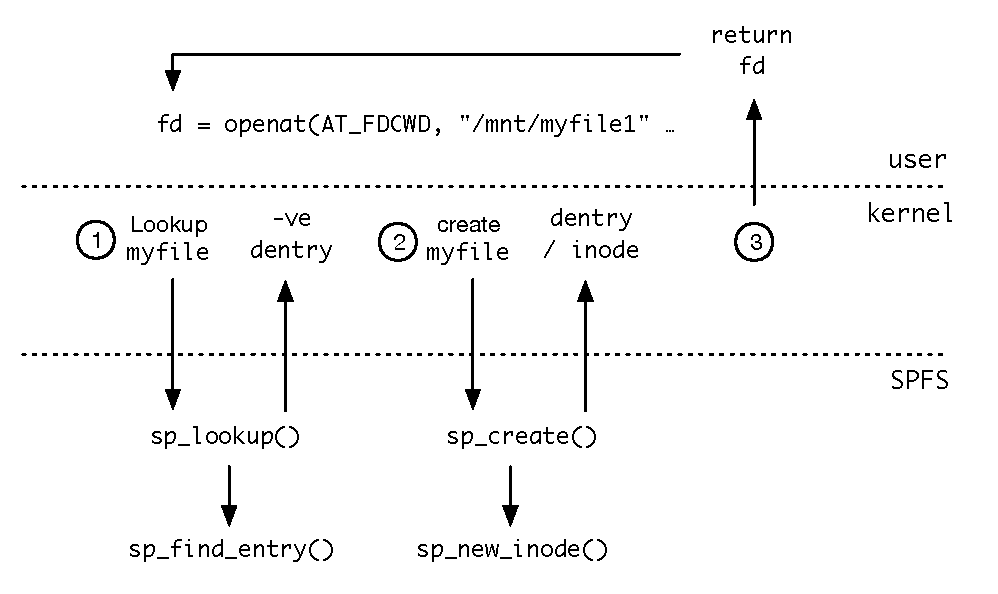
\includegraphics[scale=0.6]{figures/create-file.pdf}
	\centering
	\caption{Calls into SPFS when creating a file}
	\label{fig:create-file}
\end{figure}

\noindent
The root directory inode (now at \cf{/mnt}) was instantiated during mount processing so the kernel can query using this inode. If you recall, when a directory inode is instantiated, SPFS attaches the following operations to the \cf{i\_op} field of the Linux inode.

\begin{lstlisting}
struct inode_operations sp_dir_inops = {
    create:    sp_create,
    lookup:    sp_lookup,
    mkdir:     sp_mkdir,
    rmdir:     sp_rmdir,
    link:      sp_link,
    unlink:    sp_unlink,
};
\end{lstlisting}

\noindent
The first call that the kernel makes into SPFS when creating a file is \cf{sp\_lookup()} on the root inode (directory). It passes \cf{myfile} as an argument in addition to the directory inode and a dentry to associate with the file whether it exists or not. In turn, \cf{sp\_lookup()} calls \cf{sp\_find\_entry()} to scan the list of directory entries for the specified directory. As expected, this fails since the file does not exist. Before returning, \cf{sp\_lookup()} will call \cf{d\_splice\_alias(inode, dentry)} to create a negative dentry for \cf{myfile}. If another lookup operation were to occur on this file, the kernel now knows that the file doesn't exist. 

The kernel then calls \cf{sp\_create()} to now create the file. Once \cf{sp\_create()} creates the new file, it calls \cf{d\_instantiate(dentry, inode)} to map the entry for \cf{myfile} to the inode just created.

%------------------------------------------------------------------------------------------------------------------------------------------------------------------------

\subsection{Inside \cf{sp\_find\_entry()}}

This function is called to locate a file in the specified directory  inode. Before we show the source code, let's assume that the root directory has 96 entries. The disk structure for this would resemble figure \ref{fig:sp-filldir}.

\begin{figure}
	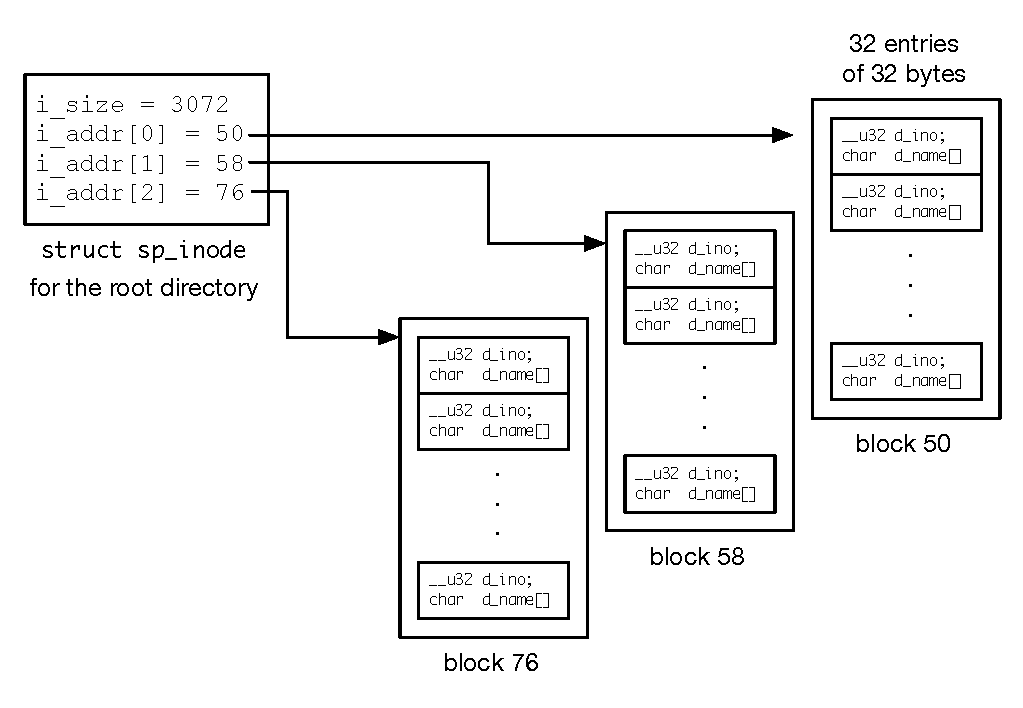
\includegraphics[scale=0.6]{figures/sp-filldir.pdf}
	\centering
	\caption{The root directory with 96 entries}
	\label{fig:sp-filldir}
\end{figure}

When the filesystem is created, we allocate block 50 as the first data block of the root inode. This is stored in the \cf{i\_addr} field of the on-disk inode. Inside the actual data block we write directory entries for ".", ".." and "lost+found". As time goes by and new files are created, we will also add them to block 50 until there is no more space. At this point, we allocated a new block (\cf{i\_addr[1] = 58}) and start adding the new directory entries in this block. And so on. A simplified form of the algorithm to search for a directory entry is:

When the filesystem is created, we allocate block 50 as the first data block of the root inode. This is stored in the \cf{i\_addr} field of the on-disk inode. Inside the actual data block we write directory entries for ".", ".." and "lost+found". As time goes by and new files are created, we will also add them to block 50 until there is no more space. At this point, we allocated a new block (\cf{i\_addr[1] = 58}) and start adding the new directory entries in this block. And so on. A simplified form of the algorithm to search for a directory entry is:
\smallskip

\noindent
\begin{algorithmic}
\For{each allocated block in the inode}
\For{all 32 directory entries in the block}
\If{the name to find matches the name in this entry}
\State return the inode number found in this entry
\EndIf
\EndFor
\EndFor
\State return 0 /* we didn't find an entry */
\end{algorithmic}

\bigskip
\noindent
The code for \cf{sp\_find\_entry()} is shown below. If the root directory had 3 allocated blocks as shown in figure \ref{fig:sp-filldir} we would require reading 3 1024 byte blocks from disk before we determine that the file does not exist.

\begin{lstlisting}
int
sp_find_entry(struct inode *dip, char *name)
{
    struct sp_inode_info    *spi = ITOSPI(dip);
    struct super_block      *sb = dip->i_sb;
    struct buffer_head      *bh;
    struct sp_dirent        *dirent;
    int                     i, blk = 0;

    printk("spfs: sp_find_entry - looking for %s (dip = %p)\n", name, dip);
    for (blk=0 ; blk < spi->i_blocks ; blk++) {
        bh = sb_bread(sb, spi->i_addr[blk]);
        dirent = (struct sp_dirent *)bh->b_data;
        for (i=0 ; i < SP_DIRS_PER_BLOCK ; i++) {
            if (strcmp(dirent->d_name, name) == 0) {
                brelse(bh);
                printk("spfs: sp_find_entry - found inum %d for %s\n",
                       dirent->d_ino, name);
                return dirent->d_ino;
            }
            dirent++;
        }
    }
    brelse(bh);
    printk("spfs: sp_find_entry - failed for %s\n", name);
    return 0;
}
\end{lstlisting}

\noindent
If the file is found, we return its inode number (allowing for a subsequent call to read the inode from disk). If it is not found, we return 0. \cf{XXX}---recall that inode number 0 is not used. For this reason.

%------------------------------------------------------------------------------------------------------------------------------------------------------------------------

\subsection{Inside \cf{sp\_create\_file()}}\label{create-file}

There are 3 different types of file creation in SPFS. Although we are covering regular file creation, we'll touch on the other two since all three operations share common paths. Let's take a look at what's needed for each but first, what is needed for all 3:

\begin{itemize}
	\item Allocate an inode on disk resulting in superblock changes.
	\item Allocate a Linux in-core inode together with its corresponding in-core SPFS inode.
	\item Update fields of both inodes to specify file properties.
	\item Write the SPFS inode to disk.
	\item Flush the superblock to disk to reflect the changes after everything else is done.
\end{itemize}

\noindent
For each of the 3 operations, there are things that are unique to the file type that we must take care of:
		
\begin{enumerate}
	\item Creating a regular file.
		\begin{itemize}
			\item Nothing. Just make sure the size of the file (\cf{i\_size}) is set to 0.
		\end{itemize}
	\item Creating a directory.
		\begin{itemize}
			\item Allocate a block for initial directory entries ("." and "..").
			\item Write this block to disk.
			\item Update inode properties ((\cf{i\_size} = 2 * (\cf{sizeof(struct sp\_direct)}, 
				\cf{i\_blocks} = 1)
		\end{itemize}
	\item Creating a symbolic link.
		\begin{itemize}
			\item Allocate a block to store the target name
			\item Write this block to disk.
			\item Update inode properties ((\cf{i\_size} = 2 * (\cf{sizeof(struct sp\_direct)}, 
				\cf{i\_blocks} = 1)
		\end{itemize}
\end{enumerate}

\noindent
Having said all of that, the core for (\cf{sp\_create\_file()} is very simple:

\begin{lstlisting}
int
sp_create(struct user_namespace *mnt_userns, struct inode *dip,
          struct dentry *dentry, umode_t mode, bool excl)
{ 
    struct inode    *inode;
    char            *name = (char *)dentry->d_name.name;
    int             error;
			
    inode = sp_new_inode(dip, dentry, S_IFREG | mode, NULL);
    if (IS_ERR(inode)) {
        error = PTR_ERR(inode);
        goto out;
    }
out:        
	return error;
}
\end{lstlisting}

\noindent
We simply rely on a call to \cf{sp\_new\_inode()} to do all of the work. The source code for \cf{sp\_mkdir()} and \cf{sp\_symlink()} is almost identical. The exception is the last argument to \cf{sp\_new\_inode()} which we will cover during the section on symlinks (\textbf{XXX}).

%------------------------------------------------------------------------------------------------------------------------------------------------------------------------

\subsection{Inside \cf{sp\_new\_inode()}}

\noindent
\begin{algorithmic}
\For{each allocated block in the inode}
\For{all 32 directory entries in the block}
\If{the name to find matches the name in this entry}
\State return the inode number found in this entry
\EndIf
\EndFor
\EndFor
\State return 0 /* we didn't find an entry */
\end{algorithmic}

%------------------------------------------------------------------------------------------------------------------------------------------------------------------------

\subsection{Inside \cf{sp\_ialloc()}}

There are two fields in the SPFS superblock (in-core and on disk) that record how many inodes have been allocated (\cf{s\_nifree} and which inodes have been allocated (the array cf{s\_inode}. 

\begin{lstlisting}
ino_t
sp_ialloc(struct super_block *sb)
{
    struct spfs_sb_info  *sbi = SBTOSPFSSB(sb);
    int                   i;

    if (sbi->s_nifree == 0) {
        printk("spfs: Out of inodes\n");
    } else {
        mutex_lock(&sbi->s_lock);
        for (i = 4 ; i < SP_MAXFILES ; i++) {
            if (sbi->s_inode[i] == SP_INODE_FREE) {
                sbi->s_inode[i] = SP_INODE_INUSE;
                sbi->s_nifree--;
                printk("spfs: sp_ialloc alloc inode %d\n", i);
                mutex_unlock(&sbi->s_lock);
                break;
            }
        }
    }
    return i;
}
\end{lstlisting}

\noindent
We check up front if any inodes are available. If not we return 0. If there is at least one inode available, we grab the SPFS superblock lock and walk through the array. As soon as we find an entry marked free, we set it to \cf{SP\_INODE\_INUSE}, drop the superblock lock and return.

%------------------------------------------------------------------------------------------------------------------------------------------------------------------------

\subsection{More on Negative dentries}

As mentioned above, when a call is made to \cf{sp\_lookup()}, the file \cf{myfile} does not exist so a negative dentry is created. In our example, the kernel follows up with a call to \cf{sp\_create()} so why is this necessary? There are times that a request will be made to test for the presence of a file as the following example shows:

\begin{lstlisting}
# [*\bfseries stat /mnt/myfile*]
stat: cannot statx '/mnt/myfile': No such file or directory
\end{lstlisting}

\noindent
In figure \ref{fig:create-file} steps 1 and 2 will be performed by the kernel to see if the file exists. This will more than likely result in the filesystem reading from disk and there could be multiple reads depending on how many directories exist. Since the file does not exist, it returns \cf{ENOENT} and retains the negative dentry.

If another \cf{stat(1)} call is made, the kernel doesn't need to call the filesystem again since it now knows that the file does not exist. And thus the role of negative dentries.

%%%%%%%%%%%%%%%%%%%%%%%%%%%%%%%%%%%%%%%%%%%%%%%%%%%%%%%%%%%%%%%%%

\section{Creating a Directory}\label{spfs-mkdir}

We covered the basics of directory creation earlier during the section \ref{create-file}. The steps performed are very straightforward. We have expanded on them here.

\begin{enumerate}
	\item Allocate a block for initial directory entries ("." and "..").
	\item Allocate an inode and set the inode properties (size, owner, group etc). The size will be set
		to 2 * \cf{sizeof(struct sp\_direct)}. Also reference the newly allocated block from within the 
		inode allocated for the new directory.
	\item Update the parent directory to add a new directory entry that points to the new file. This may
		also result in allocating a new data block for the parent directory if needed.
\end{enumerate}

\noindent
Figure \ref{fig:mkdir} is a visual presentation of how structures on disk are allocated and/or changed. In this example we assume we are creating new directory "\cf{mydir}" in the root directory (thus ".." referencing inode 2). The filesystem is empty so we only have inodes for "/" and "\cf{lost+found}" for which we have allocated data blocks 33 and 34 for the root directory and \cf{lost+found} directory entries.

\begin{figure}
	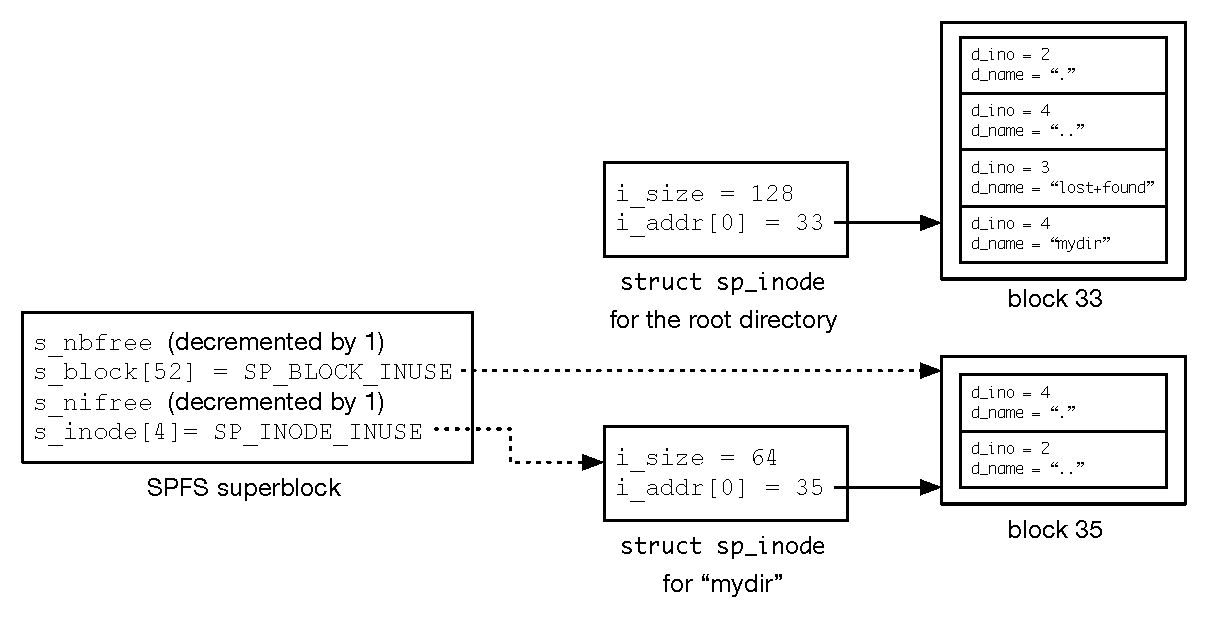
\includegraphics[scale=0.6]{figures/mkdir.pdf}
	\centering
	\caption{Structures Allocated/Modified on Disk When Creating a Directory}
	\label{fig:mkdir}
\end{figure}

\noindent
In this example:

\begin{itemize}
	\item We have allocated a new inode (number 4) for \cf{mydir}. We set the superblock \cf{s\_inode[4]}
		field to \cf{SP\_INODE\_INUSE} and decrement \cf{s\_nifree}, the number of 
		inodes free.
	\item We have allocated a new disk block (number 35) for \cf{mydir}. We set the superblock \cf{s\_block[52]}
		field to \cf{SP\_BLOCK\_INUSE} and decrement \cf{s\_nbfree}, the number of 
		blocks free.
	\item Fields of the inode for \cf{my\_dir} needs to be filled in (owner, group, size) etc. Since this is inode
		4, the inode can be found at block \cf{SP\_INODE\_BLOCK + 4} which is block 6.
\end{itemize}

\noindent
Here are the steps taken during \cf{sp\_new\_inode()} when creating a directory:

\begin{lstlisting}
} else if (S_ISDIR(mode)) {
	inode->i_blocks = 1;
	inode->i_op = &sp_dir_inops;
	inode->i_fop = &sp_dir_operations;
	inode->i_mapping->a_ops = &sp_aops;
	inode->i_size = 2 * SP_DIRENT_SIZE;

	spi->i_blocks = 1;
	blk = sp_block_alloc(sb);   /* XXX failure? */
	spi->i_addr[0] = blk;
	bh = sb_bread(sb, blk);
	if (!bh) {
		/* XXX - need to handle failure */
		return 0;
	}
	memset(bh->b_data, 0, SP_BSIZE);
	dirent = (struct sp_dirent *)bh->b_data;
	dirent->d_ino = inum;
	strcpy(dirent->d_name, ".");
	dirent++;
	dirent->d_ino = dip->i_ino;
	strcpy(dirent->d_name, "..");

	mark_buffer_dirty(bh);
	brelse(bh);
}
\end{lstlisting}

\noindent
In addition to setting fields in the Linux inode, we need to initialize the newly created SPFS inode. We call \cf{sp\_block\_alloc()} to allocate the new directory block and then call \cf{sb\_bread()} for this block. After we have set the entries for "." and ".." we mark the buffer dirty and release it so that it gets written to disk.

%--------------------------------------------------------------------------------------------------------------------------------------------------------------------------

\subsection{KGDB -- Handling the \cf{mkdir(2)} System Call}

The previous section showed how SPFS provides support for creating new directory entries. To see \cf{sp\_mkdir()} being called, a breakpoint is set and \cf{mkdir(1)} is run on the command line to create a new directory called "\cf{new-dir}" in the root directory.

A breakpoint is set in \cf{sp\_readdir()} and then the \cf{mkdir(1)} command is run. A partial stack backtrace is shown below after the breakpoint in \cf{sp\_mkdir()} is hit.

\begin{lstlisting}
(gdb) [*\bfseries bt*]
#0  [*\bfseries sp\_mkdir*] (mnt_userns=0xffffffff82a81240 <init_user_ns>, 
    dip=0xffff888103031100, dentry=0xffff888102fe3840, mode=493) 
    at /home/spate/spfs/kern/sp_dir.c:303
#1  [*\bfseries vfs\_mkdir*] (mnt_userns=0xffffffff82a81240 <init_user_ns>, 
    dir=0xffff888103031100, d
    entry=dentry@entry=0xffff888102fe3840, 
    mode=<optimized out>, mode@entry=493) 
    at fs/namei.c:3979
#2  [*\bfseries do\_mkdirat*] (dfd=dfd@entry=-100, name=0xffff88812eeea000, 
    mode=493, mode@entry=511) at fs/namei.c:4005
#3  [*\bfseries \_do\_sys\_mkdir*] (mode=<optimized out>, 
    pathname=0x7ffcb1d3287d "new-dir") at fs/namei.c:4025
    ...
\end{lstlisting}

\noindent
The \cf{dip} argument specifies the directory in which the new directory is being created and \cf{dentry} is for the newly created directory. The inode number of the parent (2) is printed out together with the name of the new directory.:

\begin{lstlisting}
(gdb) [*\bfseries p dip->i\_ino*]
$38 = 2
(gdb) [*\bfseries p dentry->d\_name.name*]
$39 = (const unsigned char *) 0xffff888102fe3878 "new-dir"
\end{lstlisting}

\noindent
Below is the path from the \cf{mkdir(2)} system call invoked by \cf{mkdir(1)} to the system call handler to the filesystem entry point. The \cf{do\_mkdirat()} system call handler can be found in \cf{fs/namei.c}. Search for \cf{SYSCALL\_DEFINE3(mkdirat}".

\small
\bigskip
\cf{mkdir(2)} $\rightarrow$ \cf{do\_mkdirat()}  $\rightarrow$ \ldots $\rightarrow$ \cf{sp\_unlink()}
%\\~\\

\bigskip
\normalsize
\noindent
For further information on the user-space implementation see TBD and for detailed handling on the VFS side of \cf{mkdir(2)} see section TBD.

%%%%%%%%%%%%%%%%%%%%%%%%%%%%%%%%%%%%%%%%%%%%%%%%%%%%%%%%%%%%%%%%

\section{Reading Directory Entries}\label{diskfs-statfs}

When we instantiate a directory inode we in \cf{sp\_read\_inode()} we attach the following operations:

\begin{lstlisting}
if (S_ISDIR(disk_ip->i_mode)) {
	inode->i_op = &sp_dir_inops;
	inode->i_fop = &sp_dir_operations;
\end{lstlisting}

\noindent
of which the function used to read directory entries can be found here:

\begin{lstlisting}
struct file_operations sp_dir_operations = {
	[*\bfseries .read           = generic\_read\_dir, XXXXXXXXXX*]
	.iterate_shared = sp_readdir,
	.fsync          = generic_file_fsync,
};
\end{lstlisting}

\noindent
The \cf{sp\_readdir()} function is called as follows:

\begin{lstlisting}
sp_readdir(struct file *f, struct dir_context *ctx)
{           
	struct inode            *ip = file_inode(f);
	struct sp_inode_info    *dip = ITOSPI(ip);
\end{lstlisting}

\noindent
We grab the Linux inode and from there we have access to the SPFS in-core inode. We may get called multiple times for a single directory. The \cf{ctx->pos} field specifies the starting positions from where we should read directory entries. It will be \cf{0} the first time called. On subsequent calls, it will be something different. This depends on the size of the user-space buffer into which we're copying data. For example, if we copy 64 entries and the buffer becomes full, SPFS will make sure that \cf{ctx->pos} will be set to the position of entry number 65 for subsequent calls.

Why do we see a \cf{struct file} as an argument and not an inode as with most other operations? Recall that inodes are shared across multiple processes each of which could be reading directory entries. {\bfseries XXX---kind of. Could still use an inode since they pass ctx so could do this above the FS. Need more info}.

To continue our discussion of \cf{sp\_readdir()} works, consider figure \ref{fig:readdir}. The directory we are reading from has 102 entries. We created 100 files in this directory and we also have "." and "..".

\begin{figure}
	\centering
	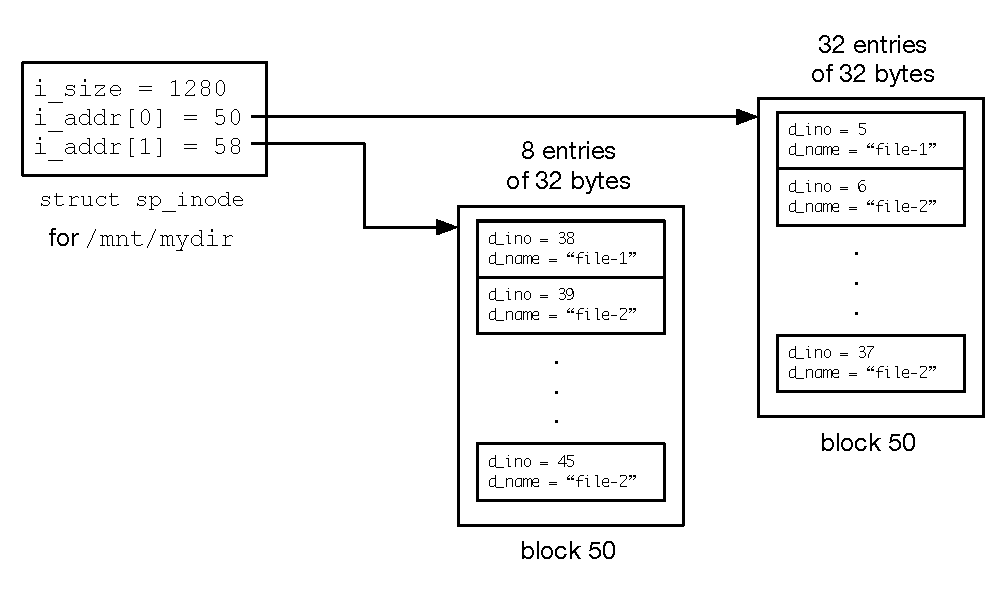
\includegraphics[scale=0.6]{figures/readdir.pdf}
	\caption{Reading from a directory with 40 entries}
	\label{fig:readdir}
\end{figure}

\noindent
As we read through directory entries we may find empty slots. For example, suppose we create files A, B and C and then delete file B. We handle this in SPFS by simply setting the \cf{i\_ino} field of the \cf{sp\_dirent} structure to \cf{0}. Therefore, the process for reading directory entires is as follows.

\begin{itemize}
	\item Walk through all entries from the requested directory.
	\item For each valid file (an inode without an inode number of 0), call the \cf{dir\_emit()}. If \cf{dir\_emit()} 
		function to copy the inode number and filename to user space ({\bfseries XXX---confirm}. If a \cf{0}
		is returned we continue reading more entries otherwise the user-space buffer so we must
		stop at this point.
	\item Increment \cf{ctx->pos} to point to the next entry.
\end{itemize}

\noindent
As we're walking through directory entries, we may need to read in multiple blocks from disk. Recall that \cf{SP\_BSIZE} is 4096 and each \cf{struct sp\_dirent} is 32 bytes so we have 64 directory entires per block.

%-------------------------------------------------------------------------------------------------------------------------------------------------------------------------

\subsection{KGDB -- Kernel Paths for Reading Directories}

\textbf{
1. small number of entries
2. much larger (100s)
}
\textbf{Fix the issue with ctx->pos before working on the larger example}

The previous section showed how SPFS provides support for reading directory entries. To see \cf{sp\_readdir()} being called, a breakpoint is set and \cf{ls(1)} is run on the command line to list the contents of two different directories, one with a small number of files and one with a much larger number. 

A breakpoint is set in \cf{sp\_readdir()} and then the \cf{ls(1)} command is run specifying one or other of the directories:

\begin{lstlisting}
(gdb) [*\bfseries ls mydir*]
file-1  file-2  file-3
(gdb) [*\bfseries ls mydir-2*]
\end{lstlisting}

\noindent
Unlike other examples in this chapter, here is the full backtrace when the breakpoint in \cf{sp\_readdir()} is hit. It shows early routines called prior to calling into routines in the Linux \cf{fs} directory.

In \cf{sp\_readdir()} the \cf{dip} argument 

\begin{lstlisting}
(gdb) [*\bfseries bt*]
#0  [*\bfseries sp\_readdir*] (f=0xffff888069f0e300, ctx=0xffffc90001063e20)
    at /home/spate/spfs/kern/sp_dir.c:130
#1  0xffffffff81403a4b in [*\bfseries iterate\_dir*] 
    (file=file@entry=0xffff888069f0e300, 
    ctx=ctx@entry=0xffffc90001063e20) 
    at fs/readdir.c:67
#2  0xffffffff81404714 in [*\bfseries \_\_do\_sys\_getdents64*] (count=32768, 
    dirent=<optimized out>, fd=<optimized out>) 
    at fs/readdir.c:369
#3  [*\bfseries \_\_se\_sys\_getdents64*] (count=32768, dirent=<optimized out>, 
    fd=<optimized out>) at fs/readdir.c:354
#4  [*\bfseries \_\_x64\_sys\_getdents64*] (regs=<optimized out>) 
    at fs/readdir.c:354
#5  0xffffffff81eaa16b in [*\bfseries do\_syscall\_x64*] (nr=<optimized out>, 
    regs=0xffffc90001063f58) at arch/x86/entry/common.c:50
#6  [*\bfseries do\_syscall\_64*] (regs=0xffffc90001063f58, nr=<optimized out>)
    at arch/x86/entry/common.c:80
#7  0xffffffff8200009b in [*\bfseries entry\_SYSCALL\_64 ()*] 
    at arch/x86/entry/entry_64.S:120
\end{lstlisting}

\noindent
The first argument specifies the directory that is being read as follows:

\begin{lstlisting}
(gdb) [*\bfseries p f->f\_path.dentry*]
$20 = (struct dentry *) 0xffff88806447e240
(gdb) [*\bfseries p \$20->d\_name.name*]
$21 = (const unsigned char *) 0xffff88806447e278 "mydir"
\end{lstlisting}

\noindent
The second argument (\cf{ctx}) specifies the offset of the directory to start reading entries from in addition to a function that should be called by the filesystem for each entry in the directory to copy the data to user-space. This function is used indirectly by first calling \cf{dir\_emit()}. You can find the \cf{filldir64()} function in \cf{fs/readdir.c}.

\begin{lstlisting}
(gdb) [*\bfseries p *ctx*]
$23 = {
  actor = 0xffffffff81404350 <filldir64>,
  pos = 0
}
\end{lstlisting}

\noindent
The breakpoint is actually hit twice. For the second time, we can see that \cf{ctx->pos} now has a different value (192).

\begin{lstlisting}
(gdb) [*\bfseries p *ctx*]
$25 = {
  actor = 0xffffffff81404350 <filldir64>,
  pos = 192
}

\end{lstlisting}

\noindent
We know that each SPFS directory entry is 32 bytes. In this directory there are 3 regular files in addition to "." and "..". Each time a directory entry is read, the offset advances by 32 bytes. \textbf{XXX -- and this is where stuff is badly broken somewhere. It works fine but needs fixing}

\bigskip
\begin{tabular}{ll}
\medskip
\textbf{File} &	\textbf{Offset}\\
\cf{.}&	0\\
\cf{..}&	32\\
\cf{file-1}&	64\\
\cf{file-2}&	96\\
\cf{file-3}&	128\\
next file&	160\\
\end{tabular}
\bigskip

\noindent
Below is the path from the \cf{getdents64(2)} system call invoked by \cf{ls(1)} to the system call handler to the filesystem entry point. The \cf{getdents()} system call handler can be found in \cf{fs/readdir.c}. Search for \cf{SYSCALL\_DEFINE3(getdents}".

\small
\bigskip
\cf{getdents64(2)} $\rightarrow$ \cf{do\_unlinkat()}  $\rightarrow$ \ldots $\rightarrow$ \cf{sp\_unlink()}
%\\~\\

\bigskip
\normalsize
\noindent
For further information on the user-space implementation see TBD and for detailed handling on the VFS side of \cf{readdir(3)} see section TBD.

%%%%%%%%%%%%%%%%%%%%%%%%%%%%%%%%%%%%%%%%%%%%%%%%%%%%%%%%%%%%%%%%

\section{Writing to a File}

To demonstrate how writing to a file works, let's copy a file which is under 3KB into an SPFS filesystem and use \cf{fsdb} to show the newly allocated file:

\begin{lstlisting}
$ [*\bfseries ls -l lorem-ipsum*]
-rw-r--r-- 1 spate spate 2972 Nov 28 22:17 lorem-ipsum
$ [*\bfseries cp lorem-ipsum /mnt*]
$ [*\bfseries umount /mnt*]
$ [*\bfseries fsdb /dev/sda*]
spfsdb > [*\bfseries i2*]

inode number 2
  i_mode     = 41ed
  i_size     = 160
  i_blocks   = 1
  i_addr[ 0] =  33
  ...

  Directory entries:
	inum[ 2], name[.]
	inum[ 2], name[..]
	inum[ 3], name[lost+found]
	inum[ 4], name[mydir]
	inum[ 5], name[lorem-ipsum]

spfsdb > [*\bfseries i5*]

inode number 5
  i_mode     = 81a4
  i_nlink    = 1
  i_uid      = 0
  i_gid      = 0
  i_size     = 2972
  i_blocks   = 3
  i_addr[ 0] =  36   i_addr[ 1] =  37   i_addr[ 2] =  38
\end{lstlisting}

\noindent
Since the block size of SPFS is 1024 bytes, the file needs 3 blocks to store the 2972 bytes of the file that is being copied. These are blocks 36, 27 and 38. Let's now look at SPFS calls that are made from the kernel to create the file and write the contents to the newly created file:

\begin{lstlisting}
sp_lookup - for lorem-ipsum
sp_find_entry - looking for lorem-ipsum (dip = 000000001d410682)
sp_find_entry - failed for lorem-ipsum
sp_lookup - lorem-ipsum not found
In sp_create for lorem-ipsum
sp_new_inode for lorem-ipsum - mode=100644
sp_ialloc allocated inode 5
In sp_diradd for lorem-ipsum (inum = 5)
sp_create - inode 000000007b2520c4 created for lorem-ipsum
sp_write_begin for inode=000000007b2520c4, off=0, len=2972
sp_get_block (inode = 000000007b2520c4, block=0)
sp_get_block - allocated blk=36 
sp_get_block (inode = 000000007b2520c4, block=1)
sp_get_block - allocated blk=37 
sp_get_block (inode = 000000007b2520c4, block=2)
sp_get_block - allocated blk=38 
sp_write_begin got page=00000000d5c0d094
sp_write_end for inode=000000007b2520c4, off=0, len=2972, 
        page=00000000d5c0d094
sp_writepage for page=00000000d5c0d094
\end{lstlisting}

\noindent
The initial calls should now be familiar but we'll cover them again in addition to calls made to write the data:

\begin{itemize}
	\item SPFS is called to lookup the file. Since this is a new file, there is no entry. This results in
		\cf{sp\_lookup()} calling \cf{d\_instantiate()} to instantiate a negative dentry.
	\item \cf{sp\_create()} is called to create the new file.
	\item The kernel then calls \cf{sp\_write\_begin()} for this file which in turn simply calls 
		\cf{block\_write\_begin()} to handle the write for us {\bfseries XXX-needs explaining}
	\item There are 3 calls to \cf{sp\_get\_block()} to allocate new blocks for the file.
	\item Need to explain \cf{sp\_write\_begin()} and \cf{sp\_write\_end()} calls and what that does.
\end{itemize}

\noindent
Since the length of the file is less than a single page (4 KB), we only see one call into SPFS to write data (the call to \cf{sp\_writepage()}. If the file that we're copying is greater than a page, we'll see multiple calls.

{\bfseries XXX---this explanation sucks. We need to explain it in much more detail or keep it simple here and reference a more detailed description somewhere else}

%-------------------------------------------------------------------------------------------------------------------------------------------------------------------------

\subsection{KGDB -- Handling the \cf{write(2)} System Call}

\textbf{XXX -- come back and add more context once page/buffer cache paths are better understood}

This section shows the path followed by the kernel in response to creating the file and writing to it:

\begin{lstlisting}
$ [*\bfseries ls -l big-lorem-ipsum *]
-rw-r--r-- 1 spate spate 5944 Apr 25 14:32 big-lorem-ipsum
$ [*\bfseries cp big-lorem-ipsum /mnt*]
\end{lstlisting}

\noindent
In the previous section, it was shown that writing to a file results in calls to the following SPFS functions after creating the file:

\begin{itemize}
	\item \cf{sp\_write\_begin()} -- prepare for write.
	\item \cf{sp\_get\_block()} -- allocate blocks.
	\item \cf{sp\_write\_end()} -- unlock the page and increase the inode size.
	\item \cf{sp\_writepage()} -- write the page to disk.
\end{itemize}

\noindent
They were only called once each as the file being created was less than a page (4096 bytes). The filesystem's \cf{write\_begin()} function is called by the the kernel to ask the filesystem to prepare to write the requested number of bytes at the given offset in the file. After a successful call to \cf{write\_begin}, and data has been copied into the allocated page, the filesystem's \cf{write\_end()} function must be called. The filesystem must unlock the page and release it, and also updating \cf{i\_size}. SPFS relies on generic kernel functions to do this. Chapter \label{vfs} discusses page/buffer cache and filesystem interactions in more detail.

Since this file is greater than a single page (4096 bytes) but also less than two pages, there will be two calls into each of these functions. Here is the stack backtrace for the first call to \cf{sp\_write\_begin()}. You can see that the kernel is requesting to write 4096 bytes and an offset of 0.

\begin{lstlisting}
(gdb)[*\bfseries  bt*]
#0  [*\bfseries sp\_write\_begin*] (file=0xffff88812ef25500, 
    mapping=0xffff888103556d78, pos=0, len=4096, 
    pagep=0xffffc900012a3ca8, fsdata=0xffffc900012a3cb0) 
    at /home/spate/spfs/kern/sp_file.c:75
#1  [*\bfseries generic\_perform\_write*] (iocb=<optimized out>, 
    i=<optimized out>) at mm/filemap.c:3779
#2  [*\bfseries \_\_generic\_file\_write\_iter*] 
    (iocb=iocb@entry=0xffffc900012a3da8, 
    from=from@entry=0xffffc900012a3d80) at mm/filemap.c:3907
#3  [*\bfseries generic\_file\_write\_iter*] (iocb=0xffffc900012a3da8, 
    from=0xffffc900012a3d80) at mm/filemap.c:3939
#4  [*\bfseries call\_write\_iter*] (iter=0xffffc900012a3d80, 
    kio=0xffffc900012a3da8, file=0xffff88812ef25500) 
    at ./include/linux/fs.h:2058
#5  [*\bfseries new\_sync\_write*] (filp=filp@entry=0xffff88812ef25500, 
    buf=buf@entry=0x7f43bce1b000 "Lorem ipsum dolor sit amet, 
    consectetur adipiscing elit. Pellentesque dignissim nisl 
    quis arcu ... Class aptent taciti so"..., len=len@entry=5944, 
    ppos=ppos@entry=0xffffc900012a3e40) at fs/read_write.c:504
#6  [*\bfseries vfs\_write*] (file=file@entry=0xffff88812ef25500, 
    buf=buf@entry=0x7f43bce1b000 "Lorem ipsum dolor sit amet, 
    nissim tempus lorem. Class aptent taciti so"..., 
    count=count@entry=5944, pos=pos@entry=0xffffc900012a3e40) 
    at fs/read_write.c:597
#7  [*\bfseries ksys\_write*] (fd=<optimized out>, 
    buf=0x7f43bce1b000 "Lorem ipsum dolor sit amet, ... 
    citi so"..., count=5944) at fs/read_write.c:650
\end{lstlisting}

\noindent
Next, SPFS will see a call to \cf{sp\_write\_end()} to information the filesystem that 4096 bytes have been copied into the page.

\begin{lstlisting}
(gdb) [*\bfseries  bt*]
#0  [*\bfseries  sp\_write\_end*] (file=0xffff88812ef25500, 
    mapping=0xffff888103556d78, pos=0, len=4096, copied=4096, 
    page=0xffffea0005277780, fsdata=0x0 <fixed_percpu_data>) 
    at /home/spate/spfs/kern/sp_file.c:93
#1  [*\bfseries  generic\_perform\_write*] (iocb=<optimized out>, 
    i=<optimized out>) at mm/filemap.c:3790
    ...
\end{lstlisting}

\noindent
The process then repeats although this time SPFS is being informed about writing 1848 bytes (the remainder of the file) at an offset of 4096:

\noindent
The process

\begin{lstlisting}
(gdb)  [*\bfseries  bt 2*]
#0  [*\bfseries  sp\_write\_begin*] (file=0xffff8881023dc800, 
    mapping=0xffff8881033b9278, pos=4096, len=1848, 
    pagep=0xffffc900011cfcd8, fsdata=0xffffc900011cfce0) 
    at /home/spate/spfs/kern/sp_file.c:75
#1  generic\_perform\_write*] (iocb=<optimized out>, 
i=<optimized out>) at mm/filemap.c:3779
\end{lstlisting}

\noindent
A final call is then made to \cf{sp\_write\_end()} informing the filesystem that 1848 bytes have been copied:

\begin{lstlisting}
(gdb)  [*\bfseries  bt 2*]
#0   [*\bfseries  sp\_write\_end*] (file=0xffff8881023dc800, 
    mapping=0xffff8881033b9278, pos=4096, len=1848, copied=1848, 
    page=0xffffea0005143940, fsdata=0x0 <fixed_percpu_data>) 
    at /home/spate/spfs/kern/sp_file.c:93
#1   [*\bfseries  generic\_perform\_write*] (iocb=<optimized out>, 
i=<optimized out>) at mm/filemap.c:3790
\end{lstlisting}

\noindent
Depending on what activity there is at the time, the file copy may not be finished from the caller's perspective. I see a shell prompt return and a short while later, a breakpoint is hit in \cf{sp\_writepage()}. Note that there is a single page passed as an argument:

\begin{lstlisting}
(gdb) [*\bfseries  bt*]
#0  [*\bfseries sp\_writepage*] (page=0xffffea0005277780, 
    wbc=0xffffc9000118bc60) 
    at /home/spate/spfs/kern/sp_file.c:105
#1  [*\bfseries \_\_writepage*] (page=page@entry=0xffffea0005277780, 
    wbc=wbc@entry=0xffffc9000118bc60, 
    data=data@entry=0xffff888103556d78) 
    at mm/page-writeback.c:2399
#2  [*\bfseries write\_cache\_pages*] (mapping=mapping@entry=0xffff888103556d78, 
    wbc=wbc@entry=0xffffc9000118bc60, 
    writepage=writepage@entry=0xffffffff812f4680 <__writepage>, 
    data=data@entry=0xffff888103556d78) 
    at mm/page-writeback.c:2334
#3  [*\bfseries generic\_writepages*] (wbc=0xffffc9000118bc60, 
    mapping=0xffff888103556d78)  
    at mm/page-writeback.c:2425
#4  [*\bfseries do\_writepages*] 
    (mapping=mapping@entry=0xffff888103556d78, 
    wbc=wbc@entry=0xffffc9000118bc60) 
    at mm/page-writeback.c:2445
#5  [*\bfseries \_\_writeback\_single\_inode*] 
    (inode=inode@entry=0xffff888103556c00, 
    wbc=wbc@entry=0xffffc9000118bc60) at fs/fs-writeback.c:1587
#6  [*\bfseries writeback\_sb\_inodes*] (sb=sb@entry=0xffff888118af5000, 
    wb=wb@entry=0xffff888100ee0860, 
    work=work@entry=0xffffc9000118be08) 
    at fs/fs-writeback.c:1870
#7  [*\bfseries \_\_writeback\_inodes\_wb*] (wb=wb@entry=0xffff888100ee0860, 
    work=work@entry=0xffffc9000118be08) 
    at fs/fs-writeback.c:1941
#8  [*\bfseries wb\_writeback*] (wb=wb@entry=0xffff888100ee0860, 
    work=work@entry=0xffffc9000118be08) 
    at fs/fs-writeback.c:2046
#9  [*\bfseries wb\_check\_background\_flush*] (wb=<optimized out>) 
    at fs/fs-writeback.c:2112
#10 [*\bfseries wb\_do\_writeback*] (wb=<optimized out>) 
    at fs/fs-writeback.c:2200
#11 [*\bfseries wb\_workfn*] (work=0xffff888100ee09f0) 
    at fs/fs-writeback.c:2227
#12 [*\bfseries process\_one\_work*] (worker=worker@entry=0xffff888119f2a180, 
    work=0xffff888100ee09f0) at kernel/workqueue.c:2289
#13 [*\bfseries worker\_thread*] (__worker=0xffff888119f2a180) 
    at kernel/workqueue.c:2436
#14 [*\bfseries kthread*] (_create=0xffff888127a279c0) at kernel/kthread.c:376
#15 [*\bfseries ret\_from\_fork*] () at arch/x86/entry/entry_64.S:306
\end{lstlisting}

\noindent
This will be followed soon after by another call to \cf{sp\_write\_page()}:

\begin{lstlisting}
(gdb) [*\bfseries bt 2*]
#0  [*\bfseries sp\_writepage*] (page=0xffffea00051ed180, 
    wbc=0xffffc900012abc60) 
    at /home/spate/spfs/kern/sp_file.c:105
#1  [*\bfseries \_\_writepage*] (page=page@entry=0xffffea00051ed180, 
    wbc=wbc@entry=0xffffc900012abc60, 
    data=data@entry=0xffff8881033b9278) 
    at mm/page-writeback.c:2399
\end{lstlisting}

\noindent
For each call, \cf{sp\_write\_page()} makes a call to \cf{block\_write\_full\_page()} to do the job of actually writing the data to disk. For further details see section \textbf{TBD}.

%%%%%%%%%%%%%%%%%%%%%%%%%%%%%%%%%%%%%%%%%%%%%%%%%%%%%%%%%%%%%%%%%

\section{Reading from a File}

Let's start with a file that is a little over 8 KB which is shown in \cf{fsdb} as follows. You can see that we need 8 blocks to store this file.

\begin{lstlisting}
spfsdb > [*\bfseries i6*]
inode number 6
  i_mode     = 81a4
  i_nlink    = 1
  i_atime    = Mon Nov 28 23:13:21 2022
  i_mtime    = Mon Nov 28 23:11:17 2022
  i_ctime    = Mon Nov 28 23:11:17 2022
  i_uid      = 0
  i_gid      = 0
  i_size     = 8916
  i_blocks   = 9
  i_addr[0] = 48 i_addr[1] = 49 i_addr[2] = 50 i_addr[3] = 51
  i_addr[4] = 52 i_addr[5] = 53 i_addr[6] = 54 i_addr[7] = 55
  i_addr[8] = 56
\end{lstlisting}

\noindent
To read the file we'll just issue a \cf{cat /mnt/big-lorem-ipsum} command to read the whole file. Here are the sequence of operations that we'll see the kernel make into SPFS to see if the file exists and then read it.

\begin{lstlisting}
sp_lookup - for big-lorem-ipsum
sp_find_entry - looking for big-lorem-ipsum 
        (dip = 00000000cec55eef)
sp_find_entry - found inum 6 for big-lorem-ipsum
sp_read_inode for ino=6
sp_read_inode gets inode = 00000000d52b9004
sp_lookup name = big-lorem-ipsum, inode = 00000000d52b9004 
        (ino=6)
sp_read_folio
sp_get_block (inode = 00000000d52b9004, block=0)
sp_get_block - NOT create blk = 48
sp_get_block (inode = 00000000d52b9004, block=1)
sp_get_block - NOT create blk = 49
sp_get_block (inode = 00000000d52b9004, block=2)
sp_get_block - NOT create blk = 50
sp_get_block (inode = 00000000d52b9004, block=3)
sp_get_block - NOT create blk = 51
sp_read_folio
sp_get_block (inode = 00000000d52b9004, block=4)
sp_get_block - NOT create blk = 52
sp_get_block (inode = 00000000d52b9004, block=5)
sp_get_block - NOT create blk = 53
sp_get_block (inode = 00000000d52b9004, block=6)
sp_get_block - NOT create blk = 54
sp_get_block (inode = 00000000d52b9004, block=7)
sp_get_block - NOT create blk = 55
sp_read_folio
sp_get_block (inode = 00000000d52b9004, block=8)
sp_get_block - NOT create blk = 56
\end{lstlisting}

\noindent
We actually do very little inside SPFS for reading files. The \cf{read\_folio} function is called and we simply invoke the generic kernel \cf{block\_read\_full\_folio()} function to do the work for us. All we need to provide is our \cf{sp\_get\_block()} function which will return a block within the file given an offset.

\begin{lstlisting}
sp_read_folio(struct file *file, struct folio *folio)
{
    printk("spfs: sp_read_folio\n");
    return block_read_full_folio(folio, sp_get_block);
}
\end{lstlisting}

\noindent
As the kernel walks through the file, it makes calls into \cf{sp\_get\_block()} to get a specific block number

\begin{lstlisting}
sp_get_block(struct inode *inode, sector_t block, 
            struct buffer_head *bh_result, int create)
{  
    ....
    } else { /* non-create path */
    phys = spi->i_addr[block];  /* sector = BLKSZ */
    printk("spfs: sp_get_block - NOT create blk = %ld\n", phys);
        map_bh(bh_result, sb, phys);
    }
\end{lstlisting}

\noindent
We are passed the block number and told this is a non-create call. Since we have the SPFS inode in-core, looking up the block given the block number is very straightforward (\cf{spi->i\_addr[block]}). The call to \cf{map\_bh()} is made to 

\begin{lstlisting}
static inline void
map_bh(struct buffer_head *bh, struct super_block *sb, 
       sector_t block)
{
	set_buffer_mapped(bh);
	bh->b_bdev = sb->s_bdev;
	bh->b_blocknr = block;
	bh->b_size = sb->s_blocksize;
}
\end{lstlisting}

\noindent
{\bfseries XXX---Need to find out what \cf{set\_buffer\_mapped()} does. Also need to walk through what the function \cf{block\_read\_full\_folio()} does.}

%%%%%%%%%%%%%%%%%%%%%%%%%%%%%%%%%%%%%%%%%%%%%%%%%%%%%%%%%%%%%%%%%

\subsection{KGDB -- Handling the \cf{read(2)} System Call}

This one will get an audible groan as you look through the stack backtrace. We start with our 2,972 byte (one page) file \cf{lorem-ipsum} and simply run the \cf{cat(1)} command on it to read all of the file's contents. Here is the long stack backtrace and, as per usual, omitting the architecture-specific system call handling portion. Note that if you are using \cf{gdb} to analyze read paths, you will likely need to unmount/mount the filesystem between experiments since a subsequent read will just get a page cache hit and not enter the filesystem.

\begin{lstlisting}
(gdb) [*\bfseries bt*]
#0  [*\bfseries sp\_read\_folio*] (file=0xffff888116625500, 
    folio=0xffffea000598a4c0)
    at /home/spate/spfs/kern/sp_file.c:112
#1  0xffffffff812f976b in [*\bfseries read\_pages*] 
    (rac=rac@entry=0xffffc90000e2fc38) at mm/readahead.c:178
#2  0xffffffff812f99d2 in [*\bfseries page\_cache\_ra\_unbounded*] (
    ractl=ractl@entry=0xffffc90000e2fc38, nr_to_read=1, 
    lookahead_size=lookahead_size@entry=32) 
    at mm/readahead.c:263
#3  0xffffffff812f9ece in [*\bfseries do\_page\_cache\_ra*] 
    (lookahead_size=<optimized out>, 
    nr_to_read=<optimized out>, ractl=0xffffc90000e2fc38) 
    at mm/readahead.c:293
#4  [*\bfseries page\_cache\_ra\_order*] (ractl=ractl@entry=0xffffc90000e2fc38, 
    ra=ra@entry=0xffff888116625598, new_order=<optimized out>, 
    new_order@entry=0) at mm/readahead.c:550
#5  0xffffffff812fa275 in [*\bfseries ondemand\_readahead*] 
    (ractl=0xffffc90000e2fc38, folio=folio@entry=0x0 
    <fixed_percpu_data>,  req_size=<optimized out>)
    at mm/readahead.c:672
#6  0xffffffff812fa59a in [*\bfseries page\_cache\_sync\_ra*] (
    ractl=ractl@entry=0xffffc90000e2fc38, 
    req_count=<optimized out>, req_count@entry=32) 
    at mm/readahead.c:699
#7  0xffffffff812eacbb in [*\bfseries page\_cache\_sync\_readahead*] 
    (req_count=32, index=0,  file=0xffff888116625500, 
    ra=0xffff888116625598, mapping=0xffff888103344678)
    at ./include/linux/pagemap.h:1234
#8  [*\bfseries filemap\_get\_pages*] (iocb=iocb@entry=0xffffc90000e2fe30, 
    iter=iter@entry=0xffffc90000e2fe08, 
    fbatch=fbatch@entry=0xffffc90000e2fcf8) at mm/filemap.c:2594
#9  0xffffffff812eb284 in [*\bfseries filemap\_read*] 
    (iocb=iocb@entry=0xffffc90000e2fe30, 
    iter=iter@entry=0xffffc90000e2fe08,  already_read=0) 
    at mm/filemap.c:2688
#10 0xffffffff812eda24 in [*\bfseries generic\_file\_read\_iter*] 
    (iocb=0xffffc90000e2fe30,  iter=0xffffc90000e2fe08) 
    at mm/filemap.c:2834
#11 0xffffffff813e5911 in [*\bfseries call\_read\_iter*] 
    (iter=0xffffc90000e2fe08, kio=0xffffc90000e2fe30, 
    file=0xffff888116625500) at ./include/linux/fs.h:2052
#12 [*\bfseries new\_sync\_read*] (filp=filp@entry=0xffff888116625500, 
    buf=buf@entry=0x7f018c5df000 <error: Cannot access memory at 
    address 0x7f018c5df000>, len=<optimized out>, 
    ppos=ppos@entry=0xffffc90000e2fed0) at fs/read_write.c:401
#13 0xffffffff813e83ba in [*\bfseries vfs\_read*] 
    (file=file@entry=0xffff888116625500, 
    buf=buf@entry=0x7f018c5df000 <error: Cannot access memory 
    at address 0x7f018c5df000>, count=count@entry=131072, 
    pos=pos@entry=0xffffc90000e2fed0) at fs/read_write.c:482
#14 0xffffffff813e8f23 in [*\bfseries ksys\_read*] (fd=<optimized out>, 
    buf=0x7f018c5df000 <error: Cannot access memory at 
    address 0x7f018c5df000>,  count=131072) 
    at fs/read_write.c:626
#15 0xffffffff813e8fc9 in [*\bfseries \_\_do\_sys\_read*] (count=<optimized out>, 
    buf=<optimized out>, fd=<optimized out>) 
    at fs/read_write.c:636
\end{lstlisting}

\noindent
\textbf{XXX -- really need to go over the read paths and mm first. I can't see anything useful in the folio structure to display. Perhaps look at other filesystems to see if they break it down}

Below is the path from the \cf{read(2)} system call invoked by \cf{cat(1)} to the system call handler to the filesystem entry point. The \cf{ksys\_read()} system call handler can be found in \cf{fs/read\_write.c}. 

\small
\bigskip
\cf{read(2)} $\rightarrow$ \cf{ksys\_read()}  $\rightarrow$ \ldots $\rightarrow$ \cf{sp\_readfolio()}
%\\~\\

\bigskip
\normalsize
\noindent
For further information on the user-space implementation see TBD and for detailed handling on the VFS side of \cf{ksys\_read(2)} see section TBD.


%%%%%%%%%%%%%%%%%%%%%%%%%%%%%%%%%%%%%%%%%%%%%%%%%%%%%%%%%%%%%%%%%

\section{Memory Mapped Files}

The filesystem is going to see similar calls from the kernel for memory mapped files as it does for reading and writing. The program from section \ref{prog-mmap} opens a file, maps it and walks through the address space one byte at a time calling \cf{putchar(2)} to write the output to \cf{stdout}.

Since we are essentially walking through the file byte by byte we will see calls into the filesystem requesting data from the start of the file and progressing throughout it. Thus, we see the following calls into SPFS where the kernel requests blocks in turn (0, 1, 2 and so on) and SPFS returns the corresponding physical block.

\begin{lstlisting}
sp_read_folio
sp_get_block (block = 0) - not create, disk blk = 48
sp_get_block (block = 1) - not create, disk blk = 49
sp_get_block (block = 2) - not create, disk blk = 50
sp_get_block (block = 3) - not create, disk blk = 51
sp_read_folio
sp_get_block (block = 4) - not create, disk blk = 52
sp_get_block (block = 5) - not create, disk blk = 53
sp_get_block (block = 6) - not create, disk blk = 54
sp_get_block (block = 7) - not create, disk blk = 55
sp_read_folio
sp_get_block (block = 8) - NOT create, blk = 56
\end{lstlisting}

\noindent
But what happens if we walk backwards through the file accessing the last byte of the file first and walking through the file to the first byte as the following modified program shows:

\begin{lstlisting}
fd = open("/mnt/big-lorem-ipsum", O_RDONLY);
fstat(fd, &st);
addr = (char *)mmap(NULL, st.st_size, PROT_READ, MAP_SHARED, 
                    fd, 0);
close(fd);

addr += st.st_size;
for (i=0 ; i <= st.st_size ;  i++) {
	putchar(*addr);
	addr--;
}
\end{lstlisting}

\noindent
We would expected blocks in the file to be accessed in reverse or close to. But this doesn't happen. Instead we see the same series of calls into SPFS. {\bfseries XXX---need to answer why but need some bigger files and explore patterns further}.

%%%%%%%%%%%%%%%%%%%%%%%%%%%%%%%%%%%%%%%%%%%%%%%%%%%%%%%%%%%%%%%%%

\section{Removing a File}

The \cf{sp\_unlink()} function removes a file (regular file, symlink, \textbf{XXX}?).

\begin{lstlisting}
int
sp_unlink(struct inode *dip, struct dentry *dentry)

{
    struct super_block      *sb = dip->i_sb;
    struct spfs_sb_info     *sbi = SBTOSPFSSB(sb);
    struct inode            *inode = dentry->d_inode;
    struct sp_inode_info    *spi = ITOSPI(inode); 
    int                     blk, i, error = -ENOENT;
    ino_t                   inum = 0;
    
    inum = sp_find_entry(dip, (char *)dentry->d_name.name);
    if (!inum) {
        goto out;
    }
    printk("spfs: In sp_unlink for %s (inum = %ld)\n",
            (char *)dentry->d_name.name, inum);
    sp_dirdel(dip, (char *)dentry->d_name.name);
        
    dip->i_ctime = dip->i_mtime = current_time(dip);
    mark_inode_dirty(dip);

    inode->i_ctime = dip->i_ctime;
    inode_dec_link_count(inode);

    /*
     * Update the superblock summaries and free any blocks
     * that this file owned.
     */

    mutex_lock(&sbi->s_lock);
    sbi->s_inode[inode->i_ino] = SP_INODE_FREE;
    sbi->s_nifree++;
    sbi->s_nbfree += spi->i_blocks;
    for (i=0 ; i < spi->i_blocks ; i++) {
        blk = spi->i_addr[i] - SP_FIRST_DATA_BLOCK;
        sbi->s_block[blk] = SP_BLOCK_FREE;
    }
    mutex_unlock(&sbi->s_lock);
    error = 0;

out:
    return error;
}
\end{lstlisting}

\textbf{XXX---change the above. unlink should not free resources. That will be done by sp\_evict\_inode()}

\noindent
One last point to consider is how to handle the directory inode \cf{i\_size} field. When a directory is created, \cf{i\_size} is set to \cf{2 * SP\_DIRENT\_SIZE} which is 64 bytes. The directory will initially have a single block of 2048 bytes. If we keep adding directory entries, we increase \cf{i\_size} by 32 bytes. Additional blocks will get allocated as needed. But what should happen when we remove a file?

figure of examples???? when to remove unused blocks? At end or in the middle? defragmentation - must be doc on this.

%------------------------------------------------------------------------------------------------------------------------------------------------------------------------

\subsection{KGDB -- Handling the \cf{unlink(2)} System Call}

The previous section showed how SPFS unlinks a file. To see \cf{sp\_unlink()} being called, a breakpoint is set and \cf{rm(1)} is run on the command line to remove a file. Below is the file hierarchy for the file \cf{lorem-ipsum} which is being removed. You can see the inode numbers of the file (7) and the parent directory (4):

\begin{lstlisting}
# [*\bfseries ls -ldi mydir*]
4 drwxr-xr-x 2 root root 96 Apr 25 15:08 mydir
# [*\bfseries ls -li mydir/lorem-ipsum *]
7 -rw-r--r-- 1 root root 2972 Apr 25 20:15 mydir/lorem-ipsum
\end{lstlisting}

\noindent
A breakpoint is set in \cf{sp\_unlink()} and then the \cf{rm(1)} is run:

\begin{lstlisting}
# [*\bfseries rm mydir/lorem-ipsum*]
\end{lstlisting}

\noindent
Here is a partial backtrace when the breakpoint in \cf{sp\_unlink()} is hit :

\begin{lstlisting}
(gdb) [*\bfseries bt*]
#0  [*\bfseries sp\_unlink*](dip=0xffff88810327df00, dentry=0xffff888102e38300)
    at /home/spate/spfs/kern/sp_dir.c:506
#1  0xffffffff813f9986 in [*\bfseries vfs\_unlink*] (mnt_userns
    =<optimized out>, dir=0xffff88810327df00, 
    dentry=dentry@entry=0xffff888102e38300, 
    delegated_inode=delegated_inode@ \
    entry=0xffffc90000e2fea0) at fs/namei.c:4196
#2  0xffffffff813ff2fe in [*\bfseries do\_unlinkat*] (dfd=dfd@entry=-100, 
    name=0xffff888100d77000) at fs/namei.c:4264
#3  0xffffffff813ff657 in [*\bfseries \_\_do\_sys\_unlinkat*](flag=<optimized out>, 
    pathname=<optimized out>, dfd=<optimized out>) 
    at fs/namei.c:4307
    ...
\end{lstlisting}

\noindent
In \cf{sp\_unlink()} the \cf{dip} argument is the directory that contains the file to be removed which is referenced by the \cf{dentry} argument. Let's check the inode number of the parent and both the name and inode number of the file to be removed.

\begin{lstlisting}
(gdb) [*\bfseries p dip->i\_ino*]
$9 = 4
(gdb) [*\bfseries p dentry->d\_name.name*]
$13 = (const unsigned char *) 0xffff888102e38338 "lorem-ipsum"
(gdb) [*\bfseries p dentry->d\_inode*]
$14 = (struct inode *) 0xffff888103279780
(gdb) [*\bfseries p \$14->i\_ino*]
$15 = 7
\end{lstlisting}

\noindent
Below is the path from the \cf{unlink(2)} system call invoked by \cf{rm(1)} to the system call handler to the filesystem entry point. The \cf{do\_unlinkat()} system call handler can be found in \cf{fs/namei.c}. Search for \cf{SYSCALL\_DEFINE3(unlinkat}".

\small
\bigskip
\cf{unlink(2)} $\rightarrow$ \cf{do\_unlinkat()}  $\rightarrow$ \ldots $\rightarrow$ \cf{sp\_unlink()}
%\\~\\

\bigskip
\normalsize
\noindent
For further information on the user-space implementation see TBD and for detailed handling on the VFS side of \cf{unlink(2)} see section TBD.

%%%%%%%%%%%%%%%%%%%%%%%%%%%%%%%%%%%%%%%%%%%%%%%%%%%%%%%%%%%%%%%

\section{Renaming a File}

I thought that rename would be a difficult operation to implement, especially when adding a directory entry in the target. But since I already have a function to add a directory entry for file creation and remove a directory entry for file removal, the \cf{sp\_rename()} implementation was nothing more than a call to both functions as follows:

\begin{lstlisting}
int
sp_rename(struct user_namespace *mnt_userns, 
          struct inode *old_dir, struct dentry *old_dentry, 
          struct inode *new_dir, struct dentry *new_dentry, 
          unsigned int flags)
{
    struct inode    *inode = d_inode(old_dentry);
    int             error;

    printk("spfs: In sp_rename %s -> %s\n", 
            old_dentry->d_name.name, new_dentry->d_name.name);

    error = sp_diradd(new_dir, new_dentry->d_name.name, 
                      inode->i_ino);
    if (error == 0) {
        sp_dirdel(old_dir, (char *)old_dentry->d_name.name);
    }
    return error;
}
\end{lstlisting}

\noindent
\textbf{XXX---at some point need to cover locking. Are both inodes locked on entry?}

%------------------------------------------------------------------------------------------------------------------------------------------------------------------

\subsection{KGDB -- Handling the \cf{rename(2)} System Call}

The previous section showed how SPFS renames a file. To see \cf{sp\_rename()} being called, a breakpoint is set in \cf{gdb} and \cf{mv(1)} is run on the command line to move a file to a different directory and with a new name. Here is the file to be moved showing its inode number (4) and the directory which has an inode number of 5:

\begin{lstlisting}
$ [*\bfseries ls -li *]
4 -rw-r--r-- 1 root root 2972 Apr 27 22:18 lorem-ipsum
3 drwxr-xr-x 2 root root   64 Apr 27 17:03 lost+found/
5 drwxr-xr-x 1 root root   64 Apr 27 22:36 mydir/
\end{lstlisting}

\noindent
A breakpoint is set in \cf{sp\_rename()} and then the \cf{mv(1)} is run as follows:

\begin{lstlisting}
# [*\bfseries mv lorem-ipsum mydir/another-name*]
\end{lstlisting}

\noindent
Here is a partial backtrace when the breakpoint in \cf{sp\_rename()} is hit :

\begin{lstlisting}
(gdb) [*\bfseries bt*]
#0  [*\bfseries sp\_rename*] (mnt_userns=0xffffffff82a81240 <init_user_ns>, 
    old_dir=0xffff888103031100, old_dentry=0xffff88810307e600, 
    new_dir=0xffff88810316a480, new_dentry=0xffff888102fe3840, 
    flags=1) at /home/spate/spfs/kern/sp_dir.c:113
#1  [*\bfseries vfs\_rename*] (rd=rd@entry=0xffffc90001263e20) 
    at fs/namei.c:4723
#2  [*\bfseries do\_renameat2*] (olddfd=olddfd@entry=-100, 
    from=<optimized out>, newdfd=newdfd@entry=-100, 
    to=to@entry=0xffff88812eee8000, flags=flags@entry=1) 
        at fs/namei.c:4874
#3  [*\bfseries \_\_do\_sys\_renameat2*] (flags=1, newname=<optimized out>, 
    newdfd=-100, oldname=0x7ffff8062872 "lorem-ipsum", 
    olddfd=-100)  at fs/namei.c:4907
    ...
\end{lstlisting}

\noindent
In \cf{sp\_rename()}, the \cf{old\_dir} argument is the directory that contains \cf{lorem-ipsum} which is referenced by the \cf{old\_dentry} argument. The \cf{new\_dir} argument is the directory to which the file is being moved to and the \cf{new\_dentry} argument is for the file in its new location. Let's check the inode numbers of both directories and both the names of the files being moved.

\begin{lstlisting}
(gdb) [*\bfseries p old\_dir->i\_ino*]
$33 = 2
(gdb) [*\bfseries p new\_dir->i\_ino*]
$34 = 5
(gdb) [*\bfseries p old\_dentry->d\_name.name*]
$35 = (const unsigned char *) 0xffff88810307e638 "lorem-ipsum"
(gdb) [*\bfseries p new\_dentry->d\_name.name*]
$36 = (const unsigned char *) 0xffff888102fe3938 "another-name"
\end{lstlisting}

\noindent
Below is the path from the \cf{rename(2)} system call invoked by \cf{rename(1)} to the system call handler to the filesystem entry point. The \cf{do\_renameat2()} system call handler can be found in \cf{fs/namei.c}. Search for \cf{SYSCALL\_DEFINE5(renameat2"}.

\small
\bigskip
\cf{rename(2)} $\rightarrow$ \cf{do\_renameat2()}  $\rightarrow$ \ldots $\rightarrow$ \cf{sp\_rename()}
%\\~\\

\bigskip
\normalsize
\noindent
For further information on the user-space implementation see TBD and for detailed handling on the VFS side of \cf{rename(2)} see section TBD.

%%%%%%%%%%%%%%%%%%%%%%%%%%%%%%%%%%%%%%%%%%%%%%%%%%%%%%%%%%%%%%%%%

\section{Other Operations}

\begin{lstlisting}
struct address_space_operations sp_aops = {
	.dirty_folio        = block_dirty_folio,
	.invalidate_folio   = block_invalidate_folio,
	.read_folio         = sp_read_folio,
	.writepage          = sp_writepage,
	.write_begin        = sp_write_begin,
	.write_end          = sp_write_end,
	.bmap               = sp_bmap
};  

struct inode_operations sp_file_inops = {
	.link   = sp_link,
	.unlink = sp_unlink,
};

struct file_operations sp_dir_operations = {
	.read           = generic_read_dir, 
	.iterate_shared = sp_readdir,
	.fsync          = generic_file_fsync,
}; 

struct file_operations sp_file_operations = {
	.fsync          = generic_file_fsync,
	.llseek         = generic_file_llseek,
	.read_iter      = generic_file_read_iter,
	.write_iter     = generic_file_write_iter,
	.mmap           = generic_file_mmap,
	.unlocked_ioctl = sp_ioctl
};
\end{lstlisting}

%%%%%%%%%%%%%%%%%%%%%%%%%%%%%%%%%%%%%%%%%%%%%%%%%%%%%%%%%%%%%%%%%

\section{Obtaining Filesystem Information via statfs}

The \cf{df(1)} command displays information about each mounted filesystem. Here is the information displayed by \cf{df} for a newly created and mounted SPFS filesystem:

\begin{lstlisting}
# [*\bfseries df -h /mnt*]
Filesystem      Size  Used Avail Use% Mounted on
/dev/sda        440K   52K  388K  12% /mnt
\end{lstlisting}

\noindent
Refer to figure \ref{fig:fslayout} for how an SPFS filesystem is laid out.

You'll see in \cf{spfs.h} that \cf{SP\_MAXBLOCKS} is 470 and  \cf{SP\_BSIZE} is 1024 and thus the size of the filesystem is 440k. The first data block starts at block 50 and blocks 50 and 51 are used for directory entries for the root directory and \cf{lost+found}. 

The \cf{df} command uses the \cf{statfs(2)} system call to gather information for each mounted filesystem. This results in a call to \cf{sp\_statfs()} to get the necessary information for a specific mount. This function is very straightforward returning some defaults and some information about the filesystem that is kept in the in-core \cf{sp\_superblock} structure.

\begin{lstlisting}
buf->f_type = SP_MAGIC;
buf->f_bsize = SP_BSIZE;
buf->f_blocks = SP_MAXBLOCKS;
buf->f_bfree = sbi->s_nbfree;
buf->f_bavail = sbi->s_nbfree; 
buf->f_files = SP_MAXFILES; 
buf->f_ffree = sbi->s_nifree;
buf->f_fsid = u64_to_fsid(huge_encode_dev(sb->s_bdev->bd_dev));
buf->f_namelen = SP_NAMELEN;
\end{lstlisting}

\noindent
Note that \cf{f\_bfree} and \cf{f\_bavail} are both set to the number of free blocks available. SPFS does not draw a distinction between the two:

\begin{itemize}
	\item \cf{f\_bfree}---Free blocks in filesystem
	\item \cf{f\_bavail}---Free blocks available to unprivileged user
\end{itemize}

\noindent
XXX it would be good to see who actually sets these differently

More complex filesystems won't use as many defaults and the filesystem size will vary as well as the block size and the number of files available (potentially). But even with more complex filesystems, such information will be held in an in-core superblock or other such structure. 

%------------------------------------------------------------------------------------------------------------------------------------------------------------------------

\subsection{KGDB -- Handling the \cf{statfs(2)} System Call}

The previous section showed how SPFS returns filesystem attributes/statistics. To see \cf{sp\_statfs()} being called, a breakpoint is set and \cf{df(1)} is run on the command line. Here is a partial backtrace when the breakpoint is hit in \cf{sp\_statfs()}:

\begin{lstlisting}
(gdb) [*\bfseries bt*]
#0  [*\bfseries sp\_statfs*] (dentry=0xffff888104f563c0, 
    buf=0xffffc90000f17da0)
    at /home/spate/spfs/kern/sp_inode.c:273
#1  0xffffffff8143349d in [*\bfseries statfs\_by\_dentry*] 
    (dentry=0xffff888104f563c0, 
    buf=buf@entry=0xffffc90000f17da0) at fs/statfs.c:66
#2  0xffffffff81433d3a in [*\bfseries vfs\_statfs*] (buf=0xffffc90000f17da0, 
    path=0xffffc90000f17d58) at fs/statfs.c:90
#3  [*\bfseries user\_statfs*] (pathname=0x55630f2edf70 "/mnt", 
    st=st@entry=0xffffc90000f17da0) at fs/statfs.c:105
#4  0xffffffff81433ded in [*\bfseries \_\_do\_sys\_statfs*] 
    (pathname=<optimized out>, 
    buf=0x7fffc5850380) at fs/statfs.c:195
    ...
\end{lstlisting}

\noindent
The first argument to \cf{sp\_statfs()} is the \cf{dentry} for the root directory of the filesystem. From this \cf{dentry} we can get its associated \cf{inode} structure and make sure it's the SPFS root directory. It should have an inode number of 2 and its name should be "/".

\begin{lstlisting}
(gdb) [*\bfseries p dentry->d\_name.name*]
$6 = (const unsigned char *) 0xffff888104f563f8 "/"
(gdb) [*\bfseries p dentry->d\_inode*]
$7 = (struct inode *) 0xffff888104d4e580
(gdb) [*\bfseries p \$7->i\_ino*]
$8 = 2
\end{lstlisting}

\noindent
Below is the path from the \cf{statfs(2)} system call invoked by \cf{df(1)} to system call handler to filesystem entry point. The \cf{user\_statfs()} system call handler can be found in \cf{fs/statfs.c}. Search for \cf{SYSCALL\_DEFINE2(statfs}"

\small
\bigskip
\cf{statfs(2)} $\rightarrow$ \cf{user\_statfs()}  $\rightarrow$ \ldots $\rightarrow$ \cf{sp\_statfs()}
%\\~\\

\bigskip
\normalsize
\noindent
For further information on the user-space implementation see \textbf{TBD} and for detailed handling on the VFS side of \cf{statfs(2)} see section \textbf{TBD}.

%%%%%%%%%%%%%%%%%%%%%%%%%%%%%%%%%%%%%%%%%%%%%%%%%%%%%%%%%%%%%%%%%

\section{Hard Links and Symbolic Links}\label{diskfs-links}

Implementing support for symbolic links turned out to be much harder than I'd ever have thought with a lot of kernel panics and confusion on my part. I'll explain the approach I took to get this working then will further discuss the different options later (section \cf{XXX}).

First I decided to keep it simple and store the symlink in a data block and read it in when requested. This is the old style way of storing symlinks since space inside the inode has generally been at a premium. With a disk-based inode where I'm storing disk blocks, I'd rather have more blocks, and therefore a larger file size, than space for a symlink since symlinks are used much less frequently. This method of storing symlinks within their own disk blocks is called "slow symlinks" due to the disk access.

But I soon ran into a problem trying to get it to work after umount/mount.

\begin{lstlisting}
static const 
struct inode_operations sysv_symlink_inode_operations = {
	.get_link   = page_get_link,
	.getattr    = sysv_getattr,
};
\end{lstlisting}

\noindent
For symlinks read 

\begin{itemize}
	\item https://www.halolinux.us/kernel-reference/lookup-of-symbolic-links.html 
	\item https://www.kernel.org/doc/Documentation/filesystems/porting.rst
	\item https://unix.stackexchange.com/questions/147535/fast-and-slow-symlinks
\end{itemize}

\noindent
When creating a new inode for a symlink, a call is made as follows:

\begin{lstlisting}
page_symlink(inode, symlink_target, slen);
\end{lstlisting}

\noindent
This kernel function gets the address space operations we attached to the new inode and calls:

\begin{lstlisting}
aops->write_begin(NULL, mapping, 0, len-1, &page, &fsdata);
memcpy(page_address(page), symname, len-1);
aops->write_end(NULL, mapping, 0, len-1, len-1, page, fsdata);
mark_inode_dirty(inode);
\end{lstlisting}

\noindent
{\bf NOTE}---you must hash an inode before making it dirty otherwise making it dirty later won't work. I was calling \cf{page\_symlink()} before calling \cf{insert\_inode\_hash()} and so the inode never gets marked dirty. This is done in sp\_new\_inode(). I set up each inode by type (reg,dir,lnk) and then call \cf{mark\_inode\_dirty()} but symlinks are different due to the call to \cf{page\_symlink()} which internally calls cf{mark\_inode\_dirty()}.

%%%%%%%%%%%%%%%%%%%%%%%%%%%%%%%%%%%%%%%%%%%%%%%%%%%%%%%%%%%%%%%%%

\section{Integration with /proc}

I had thought about implementing support for ioctls to be able to fetch SPFS-specific information. For example, I could return current open files to help with debugging. But that's a lot of work when there's already a mechanism to be able to do this and that's integration with the proc filesystem.

% fs/filesystems.c:	proc_create_single("filesystems", 0, NULL, filesystems_proc_show);

TBD 

%%%%%%%%%%%%%%%%%%%%%%%%%%%%%%%%%%%%%%%%%%%%%%%%%%%%%%%%%%%%%%%%%

\section{The SPFS \cf{fsdb} Command}

One tool that was instrumental in developing SPFS was a version of \cf{fsdb} can could analyze and print various SPFS structures such as the superblock, directory entries and inodes. Also, the ability to display blocks of data in hexadecimal and ASCII formats. This allowed me to see when data structures and data were being written to disk, to make sure inodes and data blocks were allocated and deallocated correctly. If you want to take on some of the exercises at the end of this chapter, I strongly recommend that you make enhancements to \cf{fsdb} to display any structures that you might be writing to disk. The program is less than 200 lines of code and very easy to enhance.

Here are a few commands to give you an idea of how \cf{fsdb} works. First, we run \cf{fsdb} on a partition where an SPFS filesystem resides. The \cf{h} command displays commands available:

\begin{lstlisting}
# [*\bfseries ./fsdb /dev/sda*]
spfsdb > [*\bfseries h*]
q - quit
i - display inode (e.g. "i2")
s - display superblock
r - read & display file contents (e.g. "r4")
u - undelete file (will prompt for inode)
\end{lstlisting}

\noindent
The \cf{s} command displays the superblock. We show inodes inuse/free but not blocks. That would be an easy option to add.    

\begin{lstlisting}
spfsdb > [*\bfseries s*]
Superblock contents:
  s_magic   = 0x53465053
  s_mod     = SP_FSCLEAN
  s_nifree  = 123
  s_nbfree  = 627

  i_inode[ 0] = SP_INODE_INUSE
  i_inode[ 1] = SP_INODE_INUSE
  i_inode[ 2] = SP_INODE_INUSE
  i_inode[ 3] = SP_INODE_INUSE
  ...
  i_inode[126] = SP_INODE_FREE
  i_inode[127] = SP_INODE_FREE
\end{lstlisting}

\noindent
Next the \cf{i} command is used to display inode 2. Since this is a directory we show directory entries.

\begin{lstlisting}
spfsdb > [*\bfseries i2*]
inode number 2
  i_mode     = 41ed
  i_nlink    = 4
  i_atime    = Wed Dec  7 18:26:25 2022
  i_mtime    = Wed Dec  7 18:26:25 2022
  i_ctime    = Wed Dec  7 18:26:25 2022
  i_uid      = 0
  i_gid      = 0
  i_size     = 128
  i_blocks   = 1
  i_addr[ 0] = 129 

  Directory entries:
	inum[ 2], name[.]
	inum[ 2], name[..]
	inum[ 3], name[lost+found]
	inum[ 4], name[lorem-ipsum]
\end{lstlisting}

\noindent
We can see one file (\cf{lorem-ipsum} so we display the contents of inode 4:   

\begin{lstlisting}
spfsdb > [*\bfseries i4*]
inode number 4
  i_mode     = 81a4
  i_nlink    = 1
  i_atime    = Wed Dec  7 18:26:50 2022
  i_mtime    = Wed Dec  7 18:26:50 2022
  i_ctime    = Wed Dec  7 18:26:50 2022
  i_uid      = 0
  i_gid      = 0
  i_size     = 2972
  i_blocks   = 2
  i_addr[ 0] = 131   i_addr[ 1] = 132 
\end{lstlisting}

\noindent
The file fits in 2 blocks (131 and 132) so we dump out the contents of each block. If a character is non-printable a "." is displayed. 

\begin{lstlisting}
spfsdb > [*\bfseries b131*]
0000  4c6f 7265 6d20 6970 7375 6d20 646f 6c6f   Lorem ipsum dolo
0020  6563 7465 7475 7220 6164 6970 6973 6369   ectetur adipisci
0040  6573 7175 6520 6469 676e 6973 7369 6d20   esque dignissim 
...
07e0  2076 656c 2c20 736f 6c6c 6963 6974 7564    vel, sollicitud
spfsdb > [*\bfseries b132*]
0000  2050 7261 6573 656e 7420 6174 2074 656c    Praesent at tel
0020  6f6e 7661 6c6c 6973 206e 756e 6320 7365   onvallis nunc se
0040  6e61 2e20 4165 6e65 616e 2074 656d 706f   na. Aenean tempo
...
07c0  0000 0000 0000 0000 0000 0000 0000 0000   ................
07e0  0000 0000 0000 0000 0000 0000 0000 0000   ................
\end{lstlisting}

%%%%%%%%%%%%%%%%%%%%%%%%%%%%%%%%%%%%%%%%%%%%%%%%%%%%%%%%%%%%%%%%%

\section{File Undelete}

This is a fun topic to talk about. In SPFS, we've added a file undelete option which was easy it is to implement given the simplicity of this filesystem (it only took a couple of hours to implement and longer to write about). We're  also going talk about why it gets more complicated in more sophisticated filesystems becomes when journaling capabilities to avoid the all-time-consuming full \cf{fsck}. 

We've implemented undelete as part of the SPFS \cf{fsdb} command. We're also going to \textit{cheat} by making a lot of assumptions that we will discuss. But first, let's take a look at a regular file and see what structures it impacts. Figure \ref{fig:undelete} shows a filesystem that has a file in the root filesystem called \cf{lorem-ipsum}. This regular file is stored in the root filesystem and has 2 data blocks. The superblock fields for the number of free inodes (\cf{s\_ifree}) and free blocks (\cf{s\_nbfree}) were decremented when the file was created. The superblock field for the inode allocated for \cf{lorem-ipsum}  (\cf{s\_inode[4]}) was set to \cf{SP\_INODE\_INUSE} and the superblock field for the two blocks allocated (\cf{s\_block}) were updated to show that they're in use. (\cf{SP\_BLOCK\_INUSE}).

\begin{figure}
	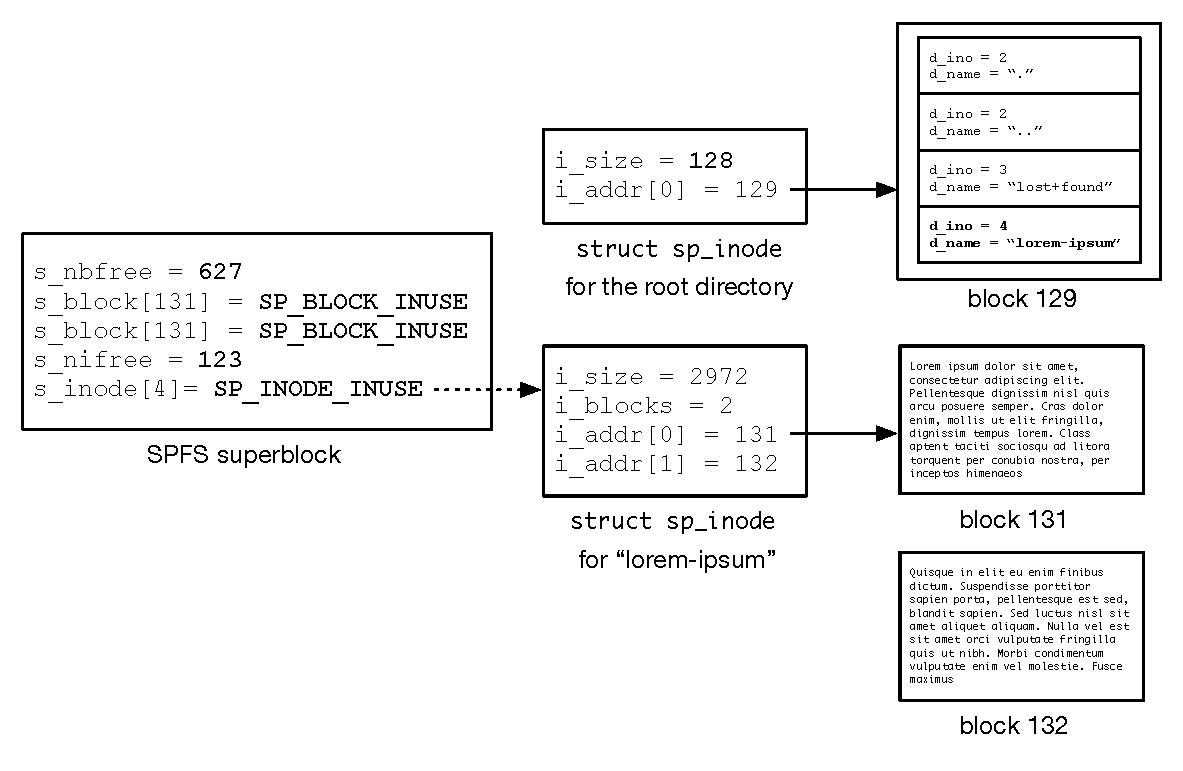
\includegraphics[scale=0.6]{figures/undelete.pdf}
	\centering
	\caption{Changes needed to implement file undelete}
	\label{fig:undelete}
\end{figure}

The reason we undelete is easy to implement is that we perform the most basic set of operations when removing the file only changing those fields in figure \ref{fig:undelete} that are shown in bold.

\begin{enumerate}
	\item Mark the inode as free in the superblock (\cf{s\_inode[4]}).
	\item For each allocated block in the deleted file, mark the block as free in the superblock \cf{s\_block}).
	\item Update superblock counts (increment number of available inodes (\cf{s\_nifree} and decrement number 
		of blocks available by 2 \cf{s\_nbfree}).
	\item Remove the directory entry for \cf{lorem-ipsum} from block 29 (from the root directory).
\end{enumerate}

\noindent
The contents of the inode are left unmodified. This includes the file size, mode, file ownership and the allocated blocks. If we were to zero the fields of the inode before deleting the file then undelete would not be possible unless this information was recorded elsewhere.

File delete won't always work. Here is the list of restrictions:

\begin{itemize}
	\item Generally speaking, the undelete operation needs to be performed as soon as possible after
		a file gets deleted. This is because the inode for the deleted file may be reallocated or the data 
		blocks owned by the deleted file may have been reused for another file.
	\item The user needs to know the node number for the file.
	\item Only regular files can be deleted.
\end{itemize}

\noindent
How does someone get the inode number? When a file is removed, we display a message which is visible by running \cf{dmesg(1)}:

\begin{lstlisting}
spfs: In sp_unlink for lorem-ipsum (inum = 4)
\end{lstlisting}

\noindent
Note however, these messages are not visible by regular users and if this were a production filesystem we wouldn't display this information at all. Therefore to make the undelete operation more user friendly, we would need a way to make this information available to regular users. One option would be to search the list of directory entries by name. This won't work "as is" since currently in \cf{sp\_dirdel()}, we delete a directory entry as follows:

\begin{lstlisting}
dirent->d_ino = 0;
dirent->d_name[0] = '\0';
mark_buffer_dirty(bh);
\end{lstlisting}

\noindent
So we don't overwrite \cf{d\_name} but we wouldn't see the filename there if we searched through possible old directory entries. We don't actually need to change the \cf{d\_name} field since having \cf{d\_ino} set to 0, we would know that the entry is free. Thus, it would be possible, given a directory, to search for all possible entries (\cf{d\_ino == 0}) and display possible names. We'll leave that an exercise to the reader if you choose to accept this mission.

%------------------------------------------------------------------------------------------------------------------------------------------------------------------------

\subsection{Enhancing Undelete}

Here are 3 possible options to consider for improving our undelete operation:

\begin{enumerate}
	\item Print the filename / inode number somewhere so that regular users can access them. Writing to
		files from a kernel module is frowned upon. Perhaps
		look at using sysfs. %(https://www.linuxjournal.com/article/8110). 
	\item Perhaps don't allocated recently deleted inodes to new files. This wouldn't completely fix the issue
		but we could maintain a pointer that references the next inode to the be allocated (initially it would
		start at 4 (just after \cf{lost+found}). 
	\item Search by name as opposed to inode number. A possible approach was described above.
\end{enumerate}

\noindent
Of course in a production system, the answer would be to maintain regular backups. We cover backups in section \ref{backups}.

%------------------------------------------------------------------------------------------------------------------------------------------------------------------------

\subsection{Why Undelete is More Complex Than you Might Think?}

This section highlights cases where undelete can get very complicated if not impossible. 

Security conscious organizations don't wish to leave data lying around on disk even if it's no longer used. Commercial filesystems such as VERITAS VxFS had options for handling this decades ago based on mount options. Deleted data blocks were zeroed before being freed. Directory entries we zeroed as part of file deletion.

In our simple undelete operation, we already stated that time is a concern. Data blocks could get reused. Inodes can be reallocated. What happens if a data block were reused and then the newer file was deleted? We could ended up with the reinstated file having data that belonged to another user. This is actually very easy to demonstrate with our simple filesystem. Perhaps a partially restored file could be useful but there are risks for sure.

The way that SPFS deletes files is not the way a production filesystem would handle delete. We would actually start by removing data blocks (last block first). This way we at least retain some structural integrity. We can mark the inode as being in process of being removed. That way, \cf{fsck} knows to continue cleaning up is the system crashes before a deletion completes. This was how we handled file deletions in VxFS which was one of the earliest transaction-based filesystems. We had the concept of "extended operations". File deletion was one such operation. Although a file can be deleted, it can remain in use for some time after the deletion completes. Only when the last reference to the file goes away can the file be deleted. Thus, this operation was marked on disk so that it could be completed during log replay (think fast version of \cf{fsck}) if the system crashes. Furthermore, when removing a file, the removal is broken up into a series of operations which are logged prior to the actual filesystem structures being modified. As highlighted above, blocks will be removed first resulting in block / extent maps need to be updated and this could be more than a simple operations as it is in SPFS. In all my time at VERITAS, I only saw one occasion when a filesystem engineer managed to undelete a file.

And at VERITAS, we had multiple backup products which did the job of "undelete" very well indeed.

%%%%%%%%%%%%%%%%%%%%%%%%%%%%%%%%%%%%%%%%%%%%%%%%%%%%%%%%%%%%%%%%%

\section{How to Test SPFS}

As I added more capabilities to SPFS, I did the usual hand testing to the point of where things seemed to work. In other words, simple unit testing and also best path testing. Then as I continued to write other sections in the book, I tried different operations and as expected, found a lot of bugs or missing functionality altogether. For example, it wasn't until I was playing with the \cf{wipe(1)} command that I realize that I hadn't implemented support for file rename. 

But hand testing is only going to reveal so many issues. A real filesystem test suite is needed to really understand how stable the filesystem is. \textbf{XXX}.

% https://sourceforge.net/p/ntfs-3g/pjd-fstest/ci/master/tree/ - try this

The \textit{fstest} test suite is a Posix conformance test suite for filesystems, originally written by Pawel Jakub Dawidek, well known for his work on ZFS for FreeBSD. I set myself a goal of getting this tests uite to run on SPFS and fix as many bugs as possible before book launch.

You can find fstest here:

\begin{table}[h]
\begin{tabular}{lcl}
\parbox[r]{0.5in}{
\includegraphics[scale=0.15]{figures/url.png}} & \parbox[l]{0.55in}{URL \arabic{urls} -- } & \parbox[l]{3in}{\cf{https://tinyurl.com/2b66w58a}}
\end{tabular}
\end{table}
\stepcounter{urls}
% https://sourceforge.net/p/ntfs-3g/pjd-fstest/ci/master/tree/

\noindent
I also have a copy that's with the SPFS source code -- XXX to try and make sure it runs / make mods etc etc. Take a look at this version. There is an SPFS.readme at the top level to show changes.

%------------------------------------------------------------------------------------------------------------------------------------------------------------------------

\subsection{Testing a Commercial Filesystem}

When I was at VERITAS working on VxFS, we had an extensive test suite that was built by engineering and for many years, we had no QA team. Engineers were expected to do all testing and obviously fix any issues found. This didn't scale forever and we found that a dedicated QA team was instrumental especially as the number of platforms and versions increased.

The test suite was divided into three main parts as follows:

\begin{itemize}
	\item Conformance -- a very large array of tests whereby different operations were tried and tests would \textit{expect}
		specific results. A simple example could be to create a file with specific attributes, then run \cf{stat(2)} and 
		compare the results returned with expected results. But these tests went far beyond POSIX-style functions as
		VxFS had a lot of features that were filesystem specific.
	\item Stress testing -- just hammer the filesystem with lots of I/Os of different sizes. It could be simply utilizing a single
		process/thread or multi-threaded.
	\item Noise testing -- another set of tests which would run and have the rug pulled out of the filesystem at random times
		to emulate a system crash to make sure that log replay would complete successfully. Noise and stress testing at the 
		same time was a particular good way to test.
\end{itemize}

\noindent
I remember one particular test suite we got from one of our OEM partners that panicked the kernel/filesystem many times. It was one of the worst pieces of code I'd ever seen and actually had a comment in the test suite that said that it was the author's first ever program in C. Therefore, he was doing everything you weren't supposed to. As a consequence, it turned out to be very useful!

We also had random testing whereby one of our QA engineers was instructed to do whatever he/she wanted to break the filesystem. That also worked very well and could be any combination of anything. Perhaps stress+noise while taking snapshots/clones or any other combination that engineers wouldn't typically think of.

%%%%%%%%%%%%%%%%%%%%%%%%%%%%%%%%%%%%%%%%%%%%%%%%%%%%%%%%%%%%%%%%%

\section{An Extended SPFS Filesystem}

Hopefully at this point, you have a good idea of how a simple filesystem works on Linux. Exploring other filesystems in detail is a great next step and that will be the goal of volume 2 of this series of books. Another path is to take the base SPFS filesystem and enhance it to add more features, remove some of the limits and explore what is possible. Here are the list of things that you could work on next. I will be doing the same once I've finished writing this book. I'll be adding blog posts about each enhancement and will make all code available on github. So either head over to my website or try to make these enhancements yourself and see how your results compare with mine. I'd also love to hear what other features you'd like to see so send me email.

A list of topics that we’ll add EPFS:

\begin{itemize}
	\item Multiple block sizes. This shouldn't be fairly straightforward assuming that all code (including the
		SPFS mkfs and fsdb commands utilize constants in \cf{spfs.h} correctly.
	\item Remove the superblock limits so there is either no limits on the number of inodes or blocks in
		the filesystem or we at least remove the basic limits that are there today.
	\item Extended attributes. A simple approach would be to use space in the inode for one or more
		attributes while understanding how the xattr interfaces work. Perhaps a list of external inodes in the 
		inode where the xattrs reside. Obviously that uses more space in the inode.
	\item A use of direct, indirect, double and triple indirect blocks allowing for much larger file sizes.
	\item Use of bitmaps for free/used inode/block lists.
	\item Quotas. Not a trivial exercise by any means. \textbf{XXX---need to look at APIs}
	\item A \cf{fsck} command to repair a damaged filesystem.
	\item Better logging. \textbf{XXX}
	\item ioctls. \textbf{XXX}
	\item Silent argument to mount\_super???
	\item superblock dirty
	\item SMP issues?
	\item get familiar with fsdb and add code to view new stuff
\end{itemize}

\noindent
Come back to this.

%%%%%%%%%%%%%%%%%%%%%%%%%%%%%%%%%%%%%%%%%%%%%%%%%%%%%%%%%%%%%%%%%

\section{Notes}

MODULE\_ALIAS\_FS
MODULE\_ALIAS\_FS is defined un linux/fs.h as follows:

\#define MODULE\_ALIAS\_FS(NAME) MODULE\_ALIAS("fs-" NAME)

Seems like the goal is to load the module automatically when you do “mount -t spfs”. So how does that work?

%%%%%%%%%%%%%%%%%%%%%%%%%%%%%%%%%%%%%%%%%%%%%%%%%%%%%%%%%%%%%%%%%

\section{debugfs?}

XXX

% https://docs.kernel.org/filesystems/debugfs.html

%%%%%%%%%%%%%%%%%%%%%%%%%%%%%%%%%%%%%%%%%%%%%%%%%%%%%%%%%%%%%%%%%

\section{Conclusion}

Previous chapters covered the path from applications using libraries and invoking system calls and going through the different kernel layers including system call handling routines and through the VFS layer before making a call into the filesystem. This chapter presented a simple but fully functional disk-based filesystem called SPFS which implements most of the VFS to filesystem functions or requests that generic kernel support functions be called.

By showing examples of \cf{gdb} stack backtraces for each of the major operations, it's possible to see the full path through the kernel into the filesystem. Exact paths can sometimes differ depending on open flags and the method of I/O being performed.

An undelete option was shown which is easy for a simple filesystem such as SPFS to implement but more complex in today's more feature rich filesystems.

Finally, testing SPFS was discussed showing how to develop test suites that can support heavy-duty commercial filesystems.

Developing a kernel-based filesystem is not trivial especially when adding enterprise capabilities such as journaling, snapshots, extended attributes and ensuring that it is highly performant. This chapter showed that it's definitely possible to build a filesystem without a huge amount of code so extending it to make it fit simple use cases, is not too difficult. But if performance is not an easy, it is possible to develop a filesystem in user-space which makes the process considerably easier. The next chapter will show his this can be done using the FUSE framework.

